% This work is licensed under the Creative Commons
% Attribution-NonCommercial-ShareAlike 4.0 International License. To view a copy
% of this license, visit http://creativecommons.org/licenses/by-nc-sa/4.0/ or
% send a letter to Creative Commons, PO Box 1866, Mountain View, CA 94042, USA.

% (c) Eric Kunze, 2019

%%%%%%%%%%%%%%%%%%%%%%%%%%%%%%%%%%%%%%%%%%%%%%%%%%%%%%%%%%%%%%%%%%%%%%%%%%%%
% Template for lecture notes and exercises at TU Dresden.
%%%%%%%%%%%%%%%%%%%%%%%%%%%%%%%%%%%%%%%%%%%%%%%%%%%%%%%%%%%%%%%%%%%%%%%%%%%%

\documentclass[ngerman, a4paper, 11pt]{report}

\usepackage[ngerman]{babel}
\usepackage{../../texmf/tex/latex/layoutMathTUD}
\usepackage[smallequationskip]{../../texmf/tex/latex/mathworkMathTUD}

\usepackage{../../texmf/tex/latex/mathoperatorsMathTUD}
\usepackage{../../texmf/tex/latex/maththeorems2MathTUD}

\usepackage{../../texmf/tex/latex/titlepageMathTUD}
\usepackage{../../texmf/tex/latex/graphicsMathTUD}

%%%%%%%%%%%%%%%%%%%%%%%%%%%%%%%%%%%%%%%%%%%%%%%%%%%%%%%%%%%%%%%%%%%
%                        TITLE STYLES                             %
%%%%%%%%%%%%%%%%%%%%%%%%%%%%%%%%%%%%%%%%%%%%%%%%%%%%%%%%%%%%%%%%%%%

\usepackage{titlesec}   % change title headings look
\usepackage{chngcntr}   % modify counters
\usepackage{relsize}    % relative font size (smaller[i], larger[i], ...)

\makeatletter
\@ifpackageloaded{opensans}{}{\usepackage[scale=1]{opensans}}
\ifx\osfamily\undefined
    \newcommand*{\osfamily}{\fontfamily{fos}\selectfont}
    \DeclareTextFontCommand{\textos}{\osfamily}
\fi
\makeatother

\newcommand{\titlefont}{\osfamily}
\newcommand{\chaptersize}{\huge}
\newcommand{\sectionsize}{\LARGE}

\renewcommand{\thepart}{\Alph{part}}

% \titleformat{<command>}[<shape>]{<format>}{<label>}{<sep>}{<before-code>}[<after-code>]
% \titlespacing*{<command>}{<left>}{<before-sep>}{<after-sep>}[<right-sep>]

%%%%%%%%% Kapitel * \\ Titel
%\titleformat{\chapter}[display]{\bfseries\titlefont\color{cddarkblue}}{\chaptersize\smaller \chaptername\;\thechapter}{-10pt}{\chaptersize\MakeUppercase}%
%\titlespacing{\chapter}{10pt}{0pt}{10pt}%

%%%%%%%%% like break but additionally framed
\titleformat{\chapter}[frame]{\bfseries\titlefont\color{cddarkblue}}{\enskip \chaptersize \smaller \chaptername\;\thechapter \enskip}{10pt}{\chaptersize\centering\MakeUppercase}%
\titlespacing{\chapter}{0pt}{0pt}{10pt}%


%%%%%%%%% chapter.section
\counterwithin{section}{chapter}%
\titleformat*{\section}{\bfseries\titlefont\sectionsize}%{\thesection}{8pt}{}%
\titlespacing{\section}{0pt}{10pt}{5pt}
\titleformat*{\subsection}{\bfseries\titlefont\sectionsize\smaller}

%%%%%%%%% section.
%\renewcommand{\thechapter}{\Roman{chapter}}
%\titlelabel{\thetitle.\quad} % "." behind section/sub... (3. instead of 3)
%\counterwithout{section}{chapter}%
%\titleformat*{\section}{\bfseries\titlefont\sectionsize}%{\thesection}{8pt}{}%
%\titleformat*{\subsection}{\bfseries\titlefont\sectionsize\smaller}

%%%%%%%%% section
%\titlelabel{\thetitle \quad} % no "." behind section/sub... (3 instead of 3.)
%\titleformat{\section}[hang]{\bfseries\titlefont\sectionsize}{\thesection}{8pt}{}%
%\titleformat*{\section}{\bfseries\titlefont\sectionsize}
%\titleformat*{\subsection}{\bfseries\titlefont\sectionsize\smaller}

%%%%%%%%%%%%%%%%%%%%%%%%%%%%%%%%%%%%%%%%%%%%%%%%%%%%%%%%%%%%%%%%%%%
%                          HIGHLIGHTING                           %
%%%%%%%%%%%%%%%%%%%%%%%%%%%%%%%%%%%%%%%%%%%%%%%%%%%%%%%%%%%%%%%%%%%
\newcommand{\begriff}[1]{\textbf{#1}}
\newcommand{\person}[1]{\textsc{#1}}

%%%%%%%%%%%%%%%%%%%%%%%%%%%%%%%%%%%%%%%%%%%%%%%%%%%%%%%%%%%%%%%%%%%
%                             COUNTER                             %
%%%%%%%%%%%%%%%%%%%%%%%%%%%%%%%%%%%%%%%%%%%%%%%%%%%%%%%%%%%%%%%%%%%
\usepackage{chngcntr}

% automatic reset of section after chapter ended 
\pretocmd{\chapter}{\setcounter{section}{0}}{}{}

% automatic reset of equation counter in each section
\pretocmd{\section}{\setcounter{equation}{0}}{}{}
%%%%%%%%%%%%%%%%%%%%%%%%%%%%%%%%%%%%%%%%%%%%%%%%%%%%%%%%%%%%%%%%%%%
%                          ENUMERATIONS                           %
%%%%%%%%%%%%%%%%%%%%%%%%%%%%%%%%%%%%%%%%%%%%%%%%%%%%%%%%%%%%%%%%%%%
\usepackage{enumerate}
\usepackage[inline]{enumitem} 		%customize label

\renewcommand{\labelitemi}{\raisebox{1pt}{\scalebox{.6}{$\blacksquare$}}}
\renewcommand{\labelitemii}{$\vartriangleright$}
\renewcommand{\labelitemiii}{--}
% Variantionen des Dreiecks als Aufzählungszeichen $\blacktriangleright$ / $\vartriangleright$ / $\triangleright$

\renewcommand{\labelenumi}{(\arabic{enumi})}
\renewcommand{\labelenumii}{\alph{enumii}.}
\renewcommand{\labelenumiii}{\roman{enumiii}.}
%%%%%%%%%%%%%%%%%%%%%%%%%%%%%%%%%%%%%%%%%%%%%%%%%%%%%%%%%%%%%%%%%%%


%%%%%%%%%%%%%%%%%%%%%%%%%%%%%%%%%%%%%%%%%%%%%%%%%%%%%%%%%%%%%%%%%%%
%                         HEADER & FOOTER                         %
%%%%%%%%%%%%%%%%%%%%%%%%%%%%%%%%%%%%%%%%%%%%%%%%%%%%%%%%%%%%%%%%%%%
\newcommand*{\rightinfo}{Vorlesung Stochastik bei Prof. Behme im Sommersemester 2019}

\usepackage{tikz}       % needed for right info
\usetikzlibrary{calc}

\usepackage{fancyhdr} 	% customize header / footer
% Add new page-style (just footer), patch \chapter command to use this page style

\fancypagestyle{myStyle}{%
    \fancyhf{} %
    \fancyfoot[C]{\thepage} %
    \renewcommand{\headrulewidth}{0pt}     % Line at the header invisible
    \renewcommand{\footrulewidth}{0pt}     % Line at the footer visible
    \fancyhead[C]{\textcolor{gray}\leftmark} %
    \fancyhead[R]{%
        \begin{tikzpicture}[overlay,remember picture]
        \node [
        fill=none,  % Farbe des Randstreifens
        text=gray,  % Textfarbe
        font=\osfamily\normalsize,  % Einstellungen für die Schrift
        inner xsep=\footskip,       % Abstand des Textes von unten
        % maximale Textbreite = Papierhöhe - 2*Abstand des Textes von unten:
        text width={\dimexpr\paperheight-2\footskip\relax},
        align=center,
        minimum height=7mm,% Breite des Randstreifens
        anchor=south west,
        rotate=90
        ]
        at ($(current page.south east)+(-10mm,0mm)$)
        {\rightinfo};
        \end{tikzpicture}%
     }
}

\fancypagestyle{rightinfo}{%
    \fancyhf{} %
    \fancyfoot[C]{\thepage} %
    \renewcommand{\headrulewidth}{0pt}     % Line at the header invisible
    \renewcommand{\footrulewidth}{0pt}     % Line at the footer visible
    \fancyhead[R]{%
        \begin{tikzpicture}[overlay,remember picture]
        \node [
        fill=none,  % Farbe des Randstreifens
        text=gray,  % Textfarbe
        font=\sffamily\normalsize,  % Einstellungen für die Schrift
        inner xsep=\footskip,       % Abstand des Textes von unten
        % maximale Textbreite = Papierhöhe - 2*Abstand des Textes von unten:
        text width={\dimexpr\paperheight-2\footskip\relax},
        align=center,
        minimum height=7mm,% Breite des Randstreifens
        anchor=south west,
        rotate=90
        ]
        at ($(current page.south east)+(-10mm,0mm)$)
        {\rightinfo};
        \end{tikzpicture}%
     }
}

%% changes pagestyle on first page of each chapter; instead of empty page the normal footer is printed
\patchcmd{\chapter}{\thispagestyle{plain}}{\thispagestyle{rightinfo}}{}{}

\pagestyle{myStyle}
\pagenumbering{arabic}

%% remember chapter-title in \leftmark and \rightmark
%\renewcommand{\chaptermark}[1]{%
%    \markboth{\chaptername
%        \ \thechapter:\ #1}{}}
%
%% remember section title in \leftmark
%\renewcommand{\sectionmark}[1]{%
%    \markright{\thesection.\ #1}{}}
%
%%change header:
%\renewcommand{\headrulewidth}{0.75pt}
%\renewcommand{\footrulewidth}{0.3pt}
%\lhead{\rightmark}%left: section-number. section-title
%\rhead{\leftmark}%right: chapter chapternumber: chapter-title

% remove page number from part{}-pages
%\let\sv@endpart\@endpart
%\def\@endpart{\thispagestyle{empty}\sv@endpart}
%%%%%%%%%%%%%%%%%%%%%%%%%%%%%%%%%%%%%%%%%%%%%%%%%%%%%%%%%%%%%%%%%%%


%%%%%%%%%%%%%%%%%%%%%%%%%%%%%%%%%%%%%%%%%%%%%%%%%%%%%%%%%%%%%%%%%%%
%                        TABLE OF CONTENTS                        %
%%%%%%%%%%%%%%%%%%%%%%%%%%%%%%%%%%%%%%%%%%%%%%%%%%%%%%%%%%%%%%%%%%%
\usepackage{tocloft}

\renewcommand{\cfttoctitlefont}{\titlefont\Huge\bfseries}
%%%%%%%%%%%%%%%%%%%%%%%%%%%%%%%%%%%%%%%%%%%%%%%%%%%%%%%%%%%%%%%%%%%

%%%%%%%%%%%%%%%%%%%%%%%%%%%%%%%%%%%%%%%%%%%%%%%%%%%%%%%%%%%%%%%%%%%
%                            LISTINGS                             %
%%%%%%%%%%%%%%%%%%%%%%%%%%%%%%%%%%%%%%%%%%%%%%%%%%%%%%%%%%%%%%%%%%%
\usepackage{listings}


\usepackage{../../texmf/tex/latex/referencesMathTUD}

%%%%%%%%%%%%%%%%%%%%%%%%%%%%%%%%%%%%%%%%%%%%%%%%%%%%%%%%%%%%%%%%%%%%%%%%%%%%

%---------------------------------------
% additional packages
%---------------------------------------

% none

%---------------------------------------
% general settings
%---------------------------------------

\name{Eric Kunze}
\matnr{Nummer}
\email{\href{mailto:eric.kunze@mailbox.tu-dresden.de}{\ttfamily eric.kunze@mailbox.tu-dresden.de}}

\modul{Stochastik}
\period{Sommersemester 2019}

%\renewcommand{\tutor}{Dr. Legrand}
%\renewcommand{\group}{Tag x. DS, (un)gerade Woche}

\lecturer{Prof. Dr. Anita Behme}
\faculty{Mathematik}
\institute{Stochastik}
\professorship{Angewandte Stochastik}

%%%%%%%%%%%%%%%%%%%%%%%%%%%%%%%%%%%%%%%%%%%%%%%%%%%%%%%%%%%%%%%%%%%%%%%%%%%%

\counterwithin{themcount}{chapter}

\renewcommand{\F}{\mathcal{F}}
\newcommand{\Ecal}{\mathcal{E}}
\renewcommand{\G}{\mathcal{G}}
\undef\folge
\NewDocumentCommand{\folge}{m O{n \in \N}}{\left( #1 \right)_{#2}}
\renewcommand{\complement}{\mathsf{C}}

\def\upmodels{\perp\!\!\!\perp}

\newcommand{\widesim}[1][2.5]{
	\mathrel{\scalebox{#1}[1]{\ensuremath{\sim}}}
}


\newcommand*{\WTheorie}{Wahrscheinlichkeitstheorie }
\newcommand*{\WMass}{Wahrscheinlichkeitsmaß }
\newcommand*{\WRaum}{Wahrscheinlichkeitsraum }
\newcommand*{\WRaeume}{Wahrscheinlichkeitsräume }
\newcommand*{\WVerteilung}{Wahrscheinlichkeitsverteilung }
\newcommand*{\Wkeit}{Wahrscheinlichkeit }
\newcommand*{\ZV}{Zufallsvariable}

%%%%%%%%%%%%%%%%%%%%%%%%%%%%%%%%%%%%%%%%%%%%%%%%%%%%%%%%%%%%%%%%%%%%%%%%%%%%


\begin{document}

\makeTUtitle
    
\tableofcontents

\setcounter{chapter}{-1}
\chapter{Einleitung}

\section*{Literatur}
\begin{itemize}[nolistsep]
    \item \textit{Georgii} : Stochastik (5. Auflage)
    \item \textit{Schilling} : Wahrscheinlichkeit
    \item \textit{Bauer} : Wahrscheinlichkeitstheorie (5. Auflage)
    \item \textit{Krengel} : Einführung in die W-Theorie und Statistik
    \item \textit{Dehling \& Haupt} : Einführung in die W-Theorie und Statistik
\end{itemize}

\section*{Was ist Stochastik ?}

Altgriechisch "Stochastikos" ($\sigma \tau  \chi \alpha \tau \iota \kappa  \zeta$) $\leadsto$ "scharfsinnig im Vermuten" % TODO

Fragestellungen stammen insbesondere aus dem Glücksspiel, heute vielmehr auch aus der Versicherungs- und Finanzmathematik - überall da, wo Zufall / Risiko / Chance auftaucht.

\subsection*{Was ist mathematische Stochastik ?}
\begin{itemize}[leftmargin=*]
    \item Beschreibt zufällige Phänomene in einer exakten Sprache. \\
    Bsp.: "Beim Würfeln erscheint jedes sechste Mal (im Schnitt) die Augenzahl 6" $\leadsto$ Gesetz der großen Zahlen
    \item lässt sich in zwei Teilgebiete unterteilen: Wahrscheinlichkeitstheorie \& Statistik \\
    Die W-Theorie beschreibt und untersucht konkret gegebene Zufallssituationen. Dagegen zieht die Statistik Schlussfolgerungen aus Beobachtungen. Dabei benötigt sie die Modelle der W-Theorie - umgekehrt benötigt auch die W-Theorie die Statistik zur Bestätigung der Modelle.
    \item In diesem Semester konzentrieren wir uns auf die Wahrscheinlichkeitstheorie.
\end{itemize}



\chapter{Grundbegriffe der Wahrscheinlichkeitstheorie}
\label{chapter_1_grundbegriffe}
\section{Wahrscheinlichkeitsräume}
\subsection*{Ergebnisraum}
Welche möglichen Ausgänge eines zufälligen Geschehens interessieren uns?
\begin{*beispiel}
    Würfeln: Augenzahl, aber nicht Lage, Fallhöhe, usw.
\end{*beispiel}

\begin{definition}[Ergebnisraum]
    Die Menge der relevanten Ergebnisse eines Zufallgeschehens nennen wir \begriff{Ergebnisraum} und bezeichnen diesen mit $\Omega$.
\end{definition}

\begin{*beispiel}
    \begin{itemize}
        \item Würfeln: $\Omega = \menge{1,2, \dots , 6}$
        \item Wartezeiten: $\Omega = \R_+ = [0,\infty)$ (also überabzählbar)
    \end{itemize}
\end{*beispiel}

\subsection*{Ereignisse}
Oft interessiert man sich gar nicht für das konkrete Ergebnis des Zufallsexperiments, sondern nur für das Eintreten gewisser Ereignisse.

\begin{*beispiel}
    Würfeln: Zahl ist $> 3$ \\
    Wartezeiten: Wartezeit ist $\leq 5$ Minuten
\end{*beispiel}

Wir wollen also Teilmengen des Ergebnisraums betrachten, d.h. Elemente von $\pows{\Omega}$ (Potenzmenge), denen eine Wahrscheinlichkeit zugeordnet werden kann d.h. welche \textit{messbar} sind.

\begin{definition}[Ereignisraum]
    Sei $\Omega \neq \emptyset$ ein Ergebnisraum und $\mathcal{F}$ eine $\sigma$-Algebra auf $\Omega$, d.h. eine Familie von Teilmengen von $\Omega$, sodass 
    \begin{enumerate}
        \item $\Omega \in \mathcal F$
        \item $A \in \mathcal{F} \follows A^\complement \in \mathcal{F}$
        \item $A_1, A_2, \dots \in \mathcal{F} \follows \bigcup_{i \geq 1} A_i \in \mathcal{F}$
    \end{enumerate}
    Dann heißt $(\Omega, \mathcal{F})$ \begriff{Ereignisraum} oder messbarer Raum.
\end{definition}

\subsection*{Wahrscheinlichkeit}
Wir ordnen nun den Ereignissen Wahrscheinlichkeiten mittels einer Abbildung $\abb{\mathbb{P}}{\mathcal{F}}{[0,1]}$
zu, sodass
\begin{enumerate}
    \item[(N)] Normierung: $\mathbb{P}(\Omega) = 1$
    \item[(A)] Additivität: Für paarweise disjunkte Ereignisse $A_1, A_2, \dots \in \mathcal{F}$ ist $\mathbb{P}\left(\bigcup_{i \geq 1} A_i\right) = \sum_{i \geq 0} \mathbb{P}(A_i)$.
\end{enumerate}

(N), (A) und die Nichtnegativität von $\mathbb{P}$ werden als Kolmogorov-Axiome bezeichnet (nach Kolmogorov: Grundbegriffe der Wahrscheinlichkeitstheorie, 1933).

\begin{definition}[Wahrscheinlichkeit]
    Sei $(\Omega, \mathcal{F})$ ein Ereignisraum und $\abb{\mathbb{P}}{\mathcal{F}}{[0,1]}$ eine Abbildung mit den Eigenschaften (N) und (A). Dann heißt $\mathbb{P}$ \begriff{Wahrscheinlichkeitsmaß} oder auch \begriff{Wahrscheinlichkeitsverteilung}.
\end{definition}

Aus der Definition folgen direkt die folgenden Eigenschaften:

\begin{satz}[Rechenregelen für Wahrscheinlichkeitsmaße] \label{satz: 1.4_rechenregeln}
    Sei $\mathbb{P}$ ein W-Maß auf einem Ereignisraum $(\Omega, \mathcal{F})$ und $A,B,A_1,A_2,\dots \in \mathcal{F}$. Dann gilt:
    \begin{enumerate}[leftmargin=*]
        \item $\mathbb{P}(\emptyset) = 0$
        \item Endliche Additivität: $\mathbb{P} (A \cup B) + \mathbb{P} (A \cap B) = \mathbb{P}(A) + \mathbb{P}(B)$ und $\mathbb{P}(A) + \mathbb{P}(A^\complement) = 1$
        \item Monotonie: $A \subseteq B \follows \mathbb{P}(A) \leq \mathbb{P}(B)$
        \item $\sigma$-Subadditivität: $\mathbb{P}\left(\bigcup_{i \geq 1} A_i \right)  \leq \sum_{i \geq 1} \mathbb{P}(A_i)$
        \item $\sigma$-Stetigkeit: Wenn $A_n \nearrow A$ (d.h. $A_1 \subseteq A_2 \subseteq \cdots$ und $A = \bigcup_{i=1}^{\infty}A_i$ ) oder $A_n \searrow A$, so gilt $\mathbb{P}(A_n) \to \mathbb{P}(A)$ für $n \to \infty$
    \end{enumerate}
\end{satz}
\begin{proof}
    siehe MINT oder Schillings Lehrbuch
\end{proof}

\begin{beispiel}
    Für einen beliebigen Ereignisraum $(\Omega, \mathcal{F})$ und ein beliebiges Element $\xi \in \Omega$ definiert
    \begin{align*}
        \delta_\xi(A) := \begin{cases} 1 & \xi \in A \\ 0 & \text{sonst} \end{cases}
    \end{align*}
    ein (degeneriertes) W-Maß auf $(\Omega, \mathcal{F})$, welches wir als \begriff{Dirac-Maß} oder Dirac-Verteilung bezeichnen.
\end{beispiel}

\begin{beispiel}
    Wir betrachten das Zufallsexperiment "Würfeln mit einem fairen, 6-seitigen Würfel" mit der Ergebnismenge $\Omega = \menge{1, \dots, 6}$ und Ereignisraum $\mathcal{F} = \pows{\Omega}$. Setzen wir aus Symmetriegründen
    \begin{align*}
        \mathbb{P}(A) = \frac{\# A}{6}
    \end{align*}
    mit $\# A = \card{A} = \text{Kardinalität}$. Dies definert ein W-Maß.
\end{beispiel}

\begin{beispiel}[Wartezeiten an der Bushaltestelle] \label{beispiel: 1_1.7_exponentialverteilung}
    Ergebnisraum $\Omega = \R_+$ und Ereignisraum Borel'sche $\sigma$-Algebra $\mathcal{F} = \mathcal{B}(\R_+)$. Ein mögliches W-Maß können wir durch
    \begin{align*}
        \mathbb{P}(A) \defeq \int_A \lambda e^{-\lambda x} \dx
    \end{align*}
    für einen Parameter $\lambda > 0$ festlegen. (offensichtlich gelten $\mathbb{P}(\Omega) = 1$ und die $\sigma$-Additivität aufgrund der $\sigma$-Additivität des Integrals). Wir bezeichnen dieses Maß als \begriff{Exponentialverteilung}. (Warum gerade dieses Maß für Wartezeiten gut geeigent ist, sehen wir später.)
\end{beispiel}

%%%%%%%%%%%%%%%%%%%%%%%%%%%%%%%%%%%%%%%%%%%%%%%%%%%%%%%%%%%%%%%%%%%%%%%%%%%%%%%%%%%%%
% TODO ÜBERARBEITEN

\begin{satz}[Konstruktion von WMaßen mit Dichten] \label{satz: 1.8_mass_mit_dichte}
    Sei $(\Omega, \ereignisF)$ ein Eriegnisraum.
    \begin{itemize}[leftmargin=*]
        \item $\Omega$ abzählbar, $\ereignisF = \pows{\Omega}$:  \\
        Sei $\rho = \left( \rho(\omega) \right)_{\omega \in \Omega}$ eine Folge in $[0,1]$ in $\sum_{\omega \in \Omega} \rho(\omega) = 1$, dann definiert
        \begin{equation*}
        \P(A) = \sum_{\omega \in A} \rho(\omega), \quad A \in \ereignisF
        \end{equation*}
        ein (diskretes) WMaß $\P$ auf $(\Omega, \ereignisF)$. $\rho$ wird als \begriff{Zähldichte} bezeichnet.
        Umgekehrt definiert jedes WMaß $\P$ auf $(\Omega, \ereignisF)$ mittels $\rho(\omega) = \P(\set{\omega}), \omega \in \Omega$ eine Folge $\rho$ mit den obigen Eigenschaften.
        \item $\Omega \subseteq \Rn, \ereignisF = \borel{\Omega}$: \\
        Sei $\abb{\rho}{\Omega}{[0, \infty)}$ eine Funktion, sodass
        \begin{enumerate}[nolistsep]
            \item $\int_{\Omega} \rho(x) \dx = 1$
            \item $\set{x \in \Omega \colon \rho(x) \leq c} \in \borel{\Omega}$ für alle $c > 0$ 
        \end{enumerate}
        dann definiert $\rho$ ein WMaß $\P$ auf $(\Omega, \ereignisF)$ durch 
        \begin{equation*}
            \P(A) = \int_{A} \rho(x) \dx = \int_{A} \rho \diff{\lambda}, \quad A \in \borel{\Omega}
        \end{equation*}
        Das Integral interpretieren wir stets als Lebesgue-Integral bzgl. Lebesgue-Maß $\lambda$.
        $\rho$ bezeichnet wir als \begriff{Dichte}, \begriff{Dichtefunktion} oder \begriff{Wahrscheinlichkeitsdichte} von $\P$ und nennen ein solches $\P$ (absolut) \begriff{stetig} (bzgl. dem Lebesgue-Maß).
    \end{itemize}
\end{satz}

\begin{proof}
    Der diskrete Fall ist klar.
    Im stetigen Fall folgt die Bahuptung aus den bekannten Eigenschaften des Lebesgue-Integrals ($\nearrow$ Schilling MINT, Lemma 8.9)
\end{proof}

\begin{*bemerkung}
    \begin{itemize}[leftmargin=*, nolistsep]
        \item Die eineindeutige Beziehung zwischen Dichte und Wahrscheinlichkeitsmaß überträgt sich nicht auf den stetigen Fall.
        \begin{itemize}[nolistsep]
            \item Nicht jedes Wahrscheinlichkeitsmaß auf $(\Omega, \borel{\Omega}), \Omega \subset \Rn$ besitzt eine Dichte.
            \item Zwei Dichtefunktionen definieren dasselbe Wahrscheinlichkeitsmaß, wenn sie sich nur auf einer Menge von Lebesgue-Maß $0$ unterscheiden.
        \end{itemize}
        \item Jede auf $\Omega \subset \Rn$ definierte Dichtefunktion $\rho$ lässt sich auf ganz $\Rn$ fortsetzen durch $\rho(x) = 0, x \notin \Omega$. Das erzeugte WMaß auf $(\Rn, \borel{\Rn})$ lässt mit den WMaß auf $(\Omega, \borel{\Omega})$ identifizieren.
        \item Mittels Dirac-Maß $\delta_{x}$ können auch jedes diskrete WMaß auf $\Omega \subset \Rn$ als WMaß auf $\Rn, \borel{\Rn}$ interpretieren:
        \begin{equation*}
            \P(A) = \sum_{\omega \in A} \rho(\omega) = \int_{A} \mathrm{d} \left( \sum_{\omega \in \Omega} \rho(\omega)\delta_{\omega} \right) \quad A \in \borel{\Rn}
        \end{equation*}
        \item stetige und diskrete WMaße lassen sich kombinieren z.B. definiert
        \begin{equation*}
            \P(A) = \frac{1}{2} \delta_{0} + \frac{1}{2} \int_{A} \one_{[0,1]}(x) \dx, A \in \borel{\R}
        \end{equation*}
        ein WMaß auf $(\R, \borel{\R})$.
    \end{itemize}
\end{*bemerkung}

Abschließend erinnern wir uns an:

\begin{satz}[Eindeutigkeitssatz für Wahrscheinlichkeitsmaße] \label{satz: 1.9_eindeutigkeitssatz}
    Sei $(\Omega, \ereignisF)$ Ereignisraum und $\P$ ein WMaß auf $(\Omega, \ereignisF)$. 
    Sei $\ereignisF = \omega(\mathcal{G})$ für ein $\cap$-stabiles Erzeugendensystem $\mathcal{G} \subset \pows{\Omega}$. 
    Dann ist $\P$ bereits durch seine Einschränkung $\P |_{\mathcal{G}}$ eindeutig bestimmt.
\end{satz}
\begin{proof}
    $\nearrow$ Schilling MINT, Satz 4.5.
\end{proof}

Insbesondere definiert z.B.
\begin{equation*}
    \P([0,a)) = \int_{0}^{a} \lambda e^{-\lambda x} \dx = 1 - e^{-\lambda a}, a > 0
\end{equation*}
bereits die Exponentialverteilung aus \cref{beispiel: 1_1.7_exponentialverteilung}.


\begin{definition}[Gleichverteilung] \label{def: 1.10_gleichverteilung}
    Ist $\Omega$ endlich, so heißt das WMaß mit konstanter Zähldichte 
    \begin{equation*}
        \rho(\omega) = \frac{1}{\abs{\Omega}}
    \end{equation*} 
    die \begriff{(diskrete) Gleichverteilung} auf $\Omega$ und wird mit $\Uni(\Omega)$ notiert (\textit{U = uniform}).
    
    Ist $\Omega \subset \Rn$ eine Borelmenge mit Lebesgue-Maß $0 < \lambda^n(\Omega) < \infty$ so heißt das WMaß auf $(\Omega, \borel(\Omega))$ mit konstanter Dichtefunktion 
    \begin{equation*}
        \rho(x) = \frac{1}{\lambda^n(\Omega)}
    \end{equation*} 
    die \begriff{(stetige)  Gleichverteilung} auf $\Omega$. 
    Sie wird ebenso mit $\Uni(\Omega)$ notiert.
\end{definition}

\subsection*{Wahrscheinlichkeitsräume}

\begin{definition}[Wahrscheinlichkeitsraum]
    Ein Tripel $(\Omega, \ereignisF, \P)$ mit $\Omega, \ereignisF$ Ereignisraum und $\P$ WMaß auf $(\Omega, \ereignisF)$, nennen wir \begriff{Wahrscheinlichkeitsraum}.
\end{definition}
\section{Zufallsvariablen}

Zufallsvariablen dienen dazu von einen gegebenen Ereignisraum $(\Omega, \ereignisF)$ zu einem Modellausschnitt $\Omega', \ereignisF'$ überzugehen. 
Es handelt sich also um Abbildungen $\abb{X}{\Omega}{\Omega'}$.
Damit wir auch jedem Ereignis in $\ereignisF'$ eine Wahrscheinlichkeit zuordnen können, benötigen wir	
\begin{equation*}
    A' \in \ereignisF' \follows X^{-1} A' \in \ereignisF		
\end{equation*}
d.h. $X$ sollte \begriff{messbar} sein.

\begin{definition}[Zufallsvariable]
    Seien $(\Omega, \ereignisF)$ und $(\Omega', \ereignisF')$ Ereignisräume. Dann heißt jede messbare Abbildung
    \begin{equation*}
        \abb{X}{\Omega}{\Omega'}
    \end{equation*}
    \begriff{Zufallsvariable} (von $(\Omega, \ereignisF)$) nach $(\Omega', \ereignisF')$/ auf $(\Omega', \ereignisF')$ oder \begriff{Zufallselement}.
\end{definition}

\begin{beispiel}
    \begin{enumerate}[leftmargin=*]
        \item Ist $\Omega$ abzählbar und $\ereignisF = \pows\Omega$, so ist jede Abbildung $\abb{X}{\Omega}{\Omega'}$ messbar und damit eine Zufallsvariable.
        \item Ist $\Omega \subset \Rn$ und $\ereignisF = \borel\Omega$, so ist jede stetige Funktion $\abb{X}{\Omega}{\R}$ messbar und damit eine Zufallsvariable.
    \end{enumerate}
\end{beispiel}

\begin{satz}
    Sei $(\Omega, \ereignisF, \P)$ ein \WRaum und $X$ eine Zufallsvariable von $(\Omega, \ereignisF)$ nach $(\Omega', \ereignisF')$. Dann definiert
    \begin{equation*}
    \P'(A') \defeq \P\left(X^{-1}(A')\right) = \P\left(\set{X \in A'}\right), \quad A' \in \ereignisF'
    \end{equation*}
    ein WMaß auf $(\Omega', \ereignisF')$, welches wir als \begriff{Wahrscheinlichkeitsverteilung von $X$ unter $\P$} bezeichnen.
\end{satz}

\begin{proof}
    Aufgrund der Messbarkeit von $X$ ist die Definition sinnvoll. Zudem gelten
    \begin{equation*}
        \P'(\Omega') = \P(X^{-1}(\Omega')) = \P(\Omega) = 1
    \end{equation*}
    und für $A_1', A_2', \dots \in \ereignisF'$ paarweise disjunkt.
    \begin{equation*}
    \begin{aligned}
        \P' \left( \bigcup_{i \geq 1} A_i' \right) 
        = \P \left(X^{-1}\left( \bigcup_{i \geq 1} A_i' \right) \right) 
        &= \P \left( \bigcup_{i \geq 1} X^{-1}(A_i') \right) \\
        &= \sum_{1 \geq 1} \P(X^{-1} A_i') \quad \text{ da auch } X^{-1}A_1', X^{-1}A_2', \dots \text{ paarweise disjunkt sind} \\
        &= \sum_{1 \geq 1} \P'(A_i)
    \end{aligned}
    \end{equation*}
    Also ist $\P'$ ein WMaß.
\end{proof}

\begin{*bemerkung}
    \begin{itemize}[leftmargin=*, nolistsep]
        \item Aus Gründen der Lesbarkeit schreiben wir in der Folge $\P (X \in A) = \P ( \menge{\omega \colon X(\omega) \in A} )$
        \item Ist $X$ die Identität, so fallen die Begriffe \WMass und \WVerteilung zusammen.
        \item In der (weiterführenden) Literatur zur \WTheorie wird oft auf die Angabe eines zugrundeliegenden WRaumes verzichtet und stattdessen eine ``Zufalsvariable mit Verteilung $\P$ auf $\Omega$'' eingeführt.
        Gemeint ist (fast) immer $X$ als Identität auf $(\Omega, \ereignisF, \P)$ mit $\ereignisF = \pows\Omega$ oder $\ereignisF = \borel\Omega$.
        \item Für die Verteilung von $X$ unter $\P$ schreibe $\P_X$ und $X \sim \P_{X}$ für die Tatsache, dass $X$ gemäß $\P_X$ verteilt ist.
    \end{itemize}
\end{*bemerkung}

\begin{definition}
    Zwei Zufallsvariablen sind \begriff{identisch verteilt}, wenn sie dieselbe Verteilung haben.
\end{definition}

Von besonderen Interesse sind für uns die Zufallsvariablen, die nach $(\R, \borel\R)$ abbilden, sogenannte \begriff{reelle Zufallsvariablen}.

Da die halboffenen Intervalle $\borel\R$ erzeugen, ist die Verteilung einer reellen Zufallsvariable durch die Werte $(-\infty, c]$, $c \in \R$ eindeutig festgelegt.

\begin{definition}[Verteilungsfunktion] \label{def: 1.16_verteilungsfunktion}
    Sei $(\R, \borel\R, \P)$ ein \WRaum, so heißt
    \begin{equation*}
        \abb{F}{\R}{[0,1]} \text{ mit } x \mapsto \P((-\infty, x))
    \end{equation*}
    \begriff{(kumulative) Verteilungsfunktion von $\P$}.    
    Ist $X$ eine reelle Zufallsvariable auf beliebigen WRaum $(\Omega, \ereignisF, \P)$, so heißt
    \begin{equation*}
        \abb{F}{\R}{[0,1]} \text{ mit } x \mapsto \P(X \leq x) = \P(X \in (-\infty, x])
    \end{equation*} % TODO everything good with the X's here?
    die (kumulative) Verteilungsfunktion von $X$.
\end{definition}

\begin{beispiel}
    $(\R, \borel\R,\P)$ mit $\P$ Exponentialverteilung mit Parameter $\lambda > 0$
    \begin{equation*}
    \P(A) = \int_{A \cap [0,\infty)}\lambda e^{-\lambda x} \dx \quad A \in \borel\R
    \end{equation*}
    Dann ist
    \begin{equation*}
    F(x) = \P((-\infty, x)) = 
    \begin{cases}
        0 &x \le 0\\
        \int_{0}^{x} \lambda e^{-\lambda y} \dy = 1 - e^{-\lambda x} &x > 0
    \end{cases}\notag
    \end{equation*}
\end{beispiel}

\begin{center}
    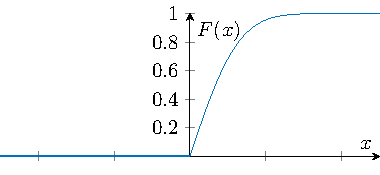
\includegraphics{./stoch_abbildungen/exponentialverteilung_verteilungsfunktion.pdf}
    \captionof{figure}{Verteilungsfunktion der Exponentialverteilung}
\end{center}

\begin{beispiel}
    Das Würfeln mit einem fairen, sechseitigen Würfel kann mittels einer reellen Zufallsvariablen
    \begin{equation*}
        \abb{X}{\menge{1,2,\dots, 6}}{\R} \mit x \mapsto x
    \end{equation*}
    modelliert werden. Es folgt als Verteilungsfunktion
    \begin{equation*}
    \begin{aligned}
    F(x) &= \P'(X \leq x) = \P(X^{-1}(-\infty,x]) = \P((-\infty,x]) \\
         &= \frac{1}{6}\sum_{i=1}^{6} \one_{\menge{i \leq x}}
    \end{aligned}
    \end{equation*}
\end{beispiel}

\begin{center}
    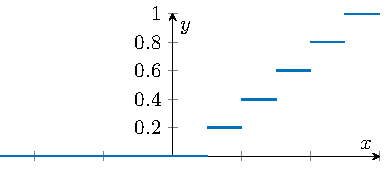
\includegraphics{./stoch_abbildungen/wuerfel_verteilungsfunktion.pdf}
    \captionof{figure}{Verteilungsfunktion des Würfelexperiments}
\end{center}

Diese Erkenntnisse lassen sich auch verallgemeinern:

\begin{satz}
    Ist $\P$ ein \WMass auf $(\R, \borel\R)$ und $F$ die zugehörige Verteilungsfunktion, so gelten
    \begin{enumerate}[nolistsep, topsep=-\parskip]
        \item $F$ ist monoton wachsend
        \item $F$ ist rechtsseitig stetig
        \item $\lim_{x\to -\infty} F(x) = 0$ und $\lim_{x\to \infty} F(x) = 1$
    \end{enumerate}
    Umgekehrt existiert zu jeder Funktion $\abb{F}{\R}{[0,1]}$ mit Eigenschaften (1) bis (3) eine reelle Zufallsvariable auf $((0,1), \borel((0,1)), \Uni((0,1))$ mit Verteilungsfunktion $F$.
\end{satz}

\begin{proof}
    Ist $F$ Verteilungsfunktion, so folgt mit \ref{satz: 1.4_rechenregeln}
    \begin{equation*}
        x \leq y \follows F(x) = \P((-\infty,x]) \overset{\ref{satz: 1.4_rechenregeln}.3}{\leq} \P((-\infty,y]) = F(y)
    \end{equation*}
    und
    \begin{equation*}
        \lim_{m \searrow c} F(x) = \lim_{m \searrow c} \P((-\infty, x]) \overset{\sigma\text{-Stetigkeit}}{=} \P((-\infty, c]) = F(c)
    \end{equation*}
    sowie
    \begin{equation*}
    \begin{aligned}
        \lim_{x\to -\infty} F(x) \overset{\ref{satz: 1.4_rechenregeln}.5}&{=} \P(\emptyset) \overset{\ref{satz: 1.4_rechenregeln}.1}{=} 0 \\
        \lim_{x\to \infty} F(x) \overset{\ref{satz: 1.4_rechenregeln}.5}&{=} \P(\R) = 1
    \end{aligned}
    \end{equation*}
    Umgekehrt wähle
    \begin{equation*}
        X(u) \defeq \inf \menge{x \in \R \colon F(x) \geq u}, \quad u \in (0,1)\\
    \end{equation*}
    Dann ist $X$ eine ``linkseitige Inverse'' von $F$ (auch \begriff{Quantilfunktion} oder \begriff{verallgemeinerte Inverse}).
    Wegen (3) gilt $-\infty < X(u) < \infty$ und zudem
    \begin{equation*}
        \menge{X \leq x} = (0, F(x)) \cap (0,1) \in \borel((0,1))
    \end{equation*}
    Da diese halboffene Mengen ein Erzeugendensystem von $\borel\R$ bilden, folgt bereits die Messbarkeit von $X$, also ist $X$ eine \ZV. Insbesondere hat die Menge $\menge{X \le x}$ gerade \person{Lebesgue}-Maß $F(x)$ und damit hat $X$ die Verteilungsfunktion $F$.
\end{proof}

\begin{korollar}
    Ist $\P$ \WMass auf $(\R, \borel\R)$ und $F$ die zugehörige Verteilungsfunktion. Dann besitzt $\P$ genau eine Dichtefunktion $\rho$, wenn $F$ stetig differenzierbar ist, denn dann gilt
    \begin{equation*}
        F(x) = \int_{0}^{x} \rho(x) \dx \quad \text{ bzw } \quad \rho(x) = F'(x)
    \end{equation*}
\end{korollar}

\begin{proof}
    Folgt aus \cref{satz: 1.8_mass_mit_dichte}, der \cref{def: 1.16_verteilungsfunktion} der Verteilungsfunktion und dem Eindeutigkeitssatz \labelcref{satz: 1.9_eindeutigkeitssatz}.
\end{proof}

\chapter{Erste Standardmodelle: Diskrete Verteilungen}
\label{chapter_2_diskreteVerteilungen}
\section{Diskrete Gleichverteilungen}

\begin{*erinnerung}[\cref{def: 1.10_gleichverteilung}]
	Ist $\Omega$ endlich, so heißt \WMass mit Zähldichte $rho(\omega) = \frac{1}{\omega}$ für $\omega \in \Omega$ \begriff{(diskrete) Gleichverteilung} auf $\Omega \leadsto \Uni(\Omega)$
\end{*erinnerung}

Es gilt das für jedes $A \in \pows(\Omega)$
\begin{equation*}
	\P(A) = \frac{\# A}{\# \Omega}
\end{equation*}

Anwendungsbeispiele sind faires Würfeln, fairer Münzwurf, Zahlenlotto, ...
\section{Urnenmodelle}

Ein ``Urnenmodell'' ist eine abstrakte Darstellung von Zufallsexperimenten, bei denen zufällig Stichproben aus einer gegebenen Menge ``gezogen'' werden.
Eine Urne ist ein Behältnis in welchem sich farbige/nummerierte Kugeln befinden, die ansonsten ununterscheidbar sind.
Aus der Urne ziehe man blind/zufällig eine oder mehrere Kugeln und notiere ihre Farbe/Zahl.

\begin{center}
    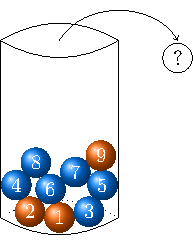
\includegraphics{./stoch_abbildungen/urne_mit_kugeln.pdf}
    \captionof{figure}{Urnenmodell mit nummerierten, farbigen Kugeln}
\end{center}

\subsection{Urnenmodell mit Zurücklegen: Multinomial-Verteilung}

Gegeben sei eine Urne mit $N$ Kugeln, verschiedenfarbig mit Farben aus $E$, wobei $\abs{E} \ge 2$ 

Man ziehe $n$ Stichproben/Kugeln, wobei nach jedem Zug die Kugel wieder zurückgelegt wird. Uns interessiert die Farbe in jedem Zug, setze also
\begin{equation*}
	\Omega = E^n \und \ereignisF = \pows\Omega 
\end{equation*}
Zur Bestimmung eines geeigneten Wahrscheinlichkeitsmaßes nummerieren wir die Kugeln mit $1,\dots, N$, so dass alle Kugeln der Farbe $a \in E$ eine Nummer aus $F_{a} \subset \menge{1,\dots, N}$ tragen. Würden wir die Nummern notieren, so wäre
\begin{equation*}
	\quer{\Omega} = \menge{1,\dots, N}^n \und \quer{\ereignisF} = \pows{\quer{\Omega}}
\end{equation*}
und wir könnten die Gleichverteilung $\quer{\P} = U(\quer{\Omega})$ als WMaß für einem einzelnen Zug verwenden. Für den Übergang zu $\Omega$ konstruieren wir  Zufallsvariablen. Die Farbe im $i$-ten Zug wird beschrieben durch
\begin{equation*}
	\bigabb{X_i}{\quer{\Omega}}{E}{\quer{\omega} = \left( \quer{\omega}_1, \dots, \quer{\omega}_n \right)}{a \enskip \text{ falls } \quer{\omega}_i \in F_a}
\end{equation*}
Der Zufallsvektor
\begin{equation*}
	\abb{X = (X_1, \dots, X_n)}{\quer{\Omega}}{\Omega}
\end{equation*}
beschreibt dann die Abfolge der Farben. Für jedes $\omega \in \Omega$ gilt dann
\begin{equation*}
	\menge{X = \omega} = F_{\omega_1} \times \cdots \times F_{\omega_n} = \bigtimes_{i=1}^{n} F_{\omega_i}
\end{equation*}
und damit
\begin{equation*}
    \P(\menge{\omega}) 
    = \quer{\P}(X^{-1}(\menge{\omega})) = \P(X=\omega)
    = \frac{\abs{F_{\omega_1}} \cdots \abs{F_{\omega_n}}}{\abs{\quer{\Omega}}}
    = \prod_{i=1}^{n} \frac{\abs{F_{\omega_i}}}{N} 
    \defqe \prod_{i=1}^{n} \rho(\omega_i)
\end{equation*}
Zähldichten, die sich als Produkt von Zähldichten schreiben lassen, werden auch als \begriff{Produktdichten} bezeichnet ($\nearrow$  \S 3 Unabhängigkeit).

Sehr oft interessiert uns bei einem Urnenexperiment nicht die Reihenfolge der gezogenen Farben, sondern nur die Anzahl der Kugeln in Farbe $a \in E$ nach $n$ Zügen. Dies entspricht
\begin{equation*}
	 \dach{\Omega} 
	 = \menge{k = (k_a)_{a \in E} \in \N_{0}^{\abs{E}} \colon \sum_{a \in E} k_a = n}
	 \und \dach{\ereignisF} = \pows{\dach{\Omega}}
\end{equation*}
Den Übergang $\Omega \to \dach{\Omega}$ beschreiben wir durch die Zufallsvariablen
\begin{equation*}
	\bigabb{Y_a(\omega)}{\Omega}{\N_{0}}%
    {\omega = (\omega_1,\dots, \omega_n)}%
    {\sum_{a \in E} \one_{\menge{a}}(\omega_i)} 
\end{equation*}
und
\begin{equation*}
	\abb{Y = (Y_a)_{a \in E}}{\Omega}{\dach{\Omega}}
\end{equation*}
Wir erhalten
\begin{equation*}
	\begin{aligned}
		\P(Y=k) &= \P(Y_a = k_a : a \in E) \\
		&= \sum_{\omega \in \Omega \colon Y(\omega) = k} \prod_{i=1}^ \rho(\omega_i)
		= \sum_{\omega \in \Omega \colon Y(\omega) = k} \prod_{a \in E} \rho(a)^{k_a} 
		= \binom{n}{\folge{k_a}[a \in E]} \prod_{a \in E} \rho(a)^{k_a}
	\end{aligned}
\end{equation*}
wobei
\begin{equation*}
	\binom{n}{(k_1 , \dots , k_l)} \defeq \begin{cases}
	\frac{n!}{k_1 ! \cdots k_l !} & \text{falls } \sum_{i=1}^l k_i = 1 \\
	0 & \text{sonst}
	\end{cases}
\end{equation*}
der Multinomialkoeffizient ist, welcher die Anzahl der Möglichkeiten beschreibt $n$ Objekte in $l$ Gruppen aufzuteilen, sodass die Gruppe $i$ gerade $k_i$ Objekte enthält.

\begin{definition}
	Sei $l \geq 2$, $p=(p_1 , \dots , p_l)$ eine Zähldichte und $n \in \N$, dann heißt die Verteilung auf 
	\begin{equation*}
		\menge{k=\folge{k_i}[i=1, \dots , l] \in \N_0^l : \sum_{i=1}^l k_i = 1}
	\end{equation*}
	mit Zähldichte
	\begin{equation*}
		m((k_1 , \dots , k_l)) = \binom{n}{k_1 , \dots , k_l} \prod_{i=1}^l p_i^{k_i}
	\end{equation*}
	\begriff{Mulitnomialverteilung} mit Parametern $n$ und $p$. Wir schreiben auch $\Multi(n,p)$.
\end{definition}

\begin{beispiel}
	Eine Urne enthalte nur schwarze (``1'') und weiße (``0'') Kugeln ($E = \menge{0,1}$) und es sei $\rho(1) = p$ gerade die Proportion der schwarzen Kugeln (Wahrscheinlichkeit bei einem Zug schwarz zu ziehen). Dann ist die Wahrscheinlichkeit in $n$ Zügen $k$-mal schwarz zu ziehen
	\begin{equation*}
		\binom{n}{k} \prod_{i=0,1} \rho(i)^{k_i} = \binom{n}{k} *p^k * (1-p)^{n-k}
	\end{equation*}
	Ein solches (wiederholtes) Experiment mit nur zwei möglichen Ergebnissen und feste Wahrscheinlichkeit $p \in [0,1]$ nennen wir auch (wiederholtes) \person{Bernoulli}-Experiment.
\end{beispiel}

\begin{definition}
	Sei $p \in [0,1]$ und $n \in \N$, dann heißt die Verteilung mit Zähldichte
	\begin{equation*}
		\rho(k) = \binom{n}{k} p^k (1-p)^{n-k} \qquad k \in \menge{0, 1 , \dots , n}
	\end{equation*}
	\begriff{Binomialverteilung} auf $\menge{0, \dots, n}$ mit Parameter $p$ (Erfolgswahrscheinlichkeit). Wir schreiben auch $\Bin(n,p)$. Im Fall $n=1$ nennen wir die Verteilung mit Zähldichte
	\begin{equation*}
		\rho(0) = 1-p \quad \rho(1) = p
	\end{equation*}
	auch \begriff{Bernoulliverteilung} mit Parameter $p$ und schreiben $\Bernoulli(p)$.
\end{definition}

\subsection{Urnenmodell ohne Zurücklegen: Hypergeometrische Verteilung}
Gegeben sei ein Urne mit $N$ Kugeln verschiedener Farben aus $E$ mit $\card{E} \geq 2$. Es werden $n \leq N$ Stichproben entnommen, wobei die gezogenen Kugeln nicht in die Urne zurückgelegt werden.

\begin{beispiel}
	Eine Urne enthalte $S$ schwarze (``1'') und $W$ weiße (``0'') Kugeln, d.h. $E = \menge{0,1}$ und $S+W=N$. Dann ist die Wahrscheinlichkeit in $n$ Zügen ohne Zurücklegen gerade $s$ schwarze und $w$ weiße Kugeln zu ziehen
	\begin{equation*}
		\rho(s) = \frac{\binom{W}{w} * \binom{S}{s}}{\binom{N}{n}} \qquad 0 \leq s \leq S, 0 \leq w \leq W, s+w=n, S+W=N
	\end{equation*}
\end{beispiel}

\begin{definition}
	Seien $N \in \N, W \leq N, n \leq N$. Dann heißt die Verteilung auf $\menge{0, \dots , n}$ mit Zähldichte 
	\begin{equation*}
		\rho(w) = \frac{\binom{W}{w} * \binom{N-W}{n-w}}{\binom{N}{n}} \qquad w = \max\menge{0 , n-N+W} , \dots \min\menge{W,n}
	\end{equation*}
	\begriff{Hypergeometrische Verteilung} mit Parametern $N,W$ und $n$. Wir schreiben auch $\Hyper(N,W,n)$.
\end{definition}
\section{Poisson-Approximation und -Verteilung}

$\Bin(n,p)$ ist zwar explizit und elementar definiert, jedoch für große $n$ mühsam auszuwerten. Für seltene Ereignisse ($n$ groß, $p$ klein) kann man daher eher den folgenden Satz anwenden.

\begin{satz}[Poisson-Approximation]
	Sei $\lambda > 0$ und $\folge{p_n}$ eine Folge in $[0,1]$ mit
	\begin{equation*}
		n*p_n \to \lambda,\quad n \to \infty
	\end{equation*}
	Dann gilt für alle $k \in \N_0$ für die Zähldichte der $\Bin(n,p_n)$-Verteilung
	\begin{equation*}
		\lim_{n \to \infty} \binom{n}{k} p_n^k (1-p_n)^{n-k} = e^{-\lambda} \frac{\lambda^k}{k!}
	\end{equation*}
\end{satz}
\begin{proof}
	Sei $k \in \N_{0}$ fix, dann
	\begin{equation*}
		\binom{n}{k} = \frac{n!}{k!(n-k)!} 
		= \frac{n^k}{k!}\frac{n(n-1)\cdots(n-k+1)}{n^k}
		= \frac{n^k}{k!}\cdot 1 \cdot (1-\frac{1}{n}\cdots \frac{k-1}{n})
		\overset{n \to \infty}{\widesim} \frac{n^k}{k!}
	\end{equation*}
	wobei $a(l) \overset{n \to \infty}{\sim} b(l) \Leftrightarrow \frac{a(l)}{b(l)} \xrightarrow{n\to \infty} 1$. Damit gilt
	\begin{equation*}
	\begin{aligned}
		\binom{n}{k}p^k (1-p)^{n-k} \overset{n \to \infty}&{\widesim} \frac{n^k}{k!}p_n^k(1-p_n)^{n-k}\\
		\overset{n \to \infty}&{\widesim} \frac{\lambda^k}{k!}(1-p_n)^n
		= \frac{\lambda^n}{k!}\brackets{1 - \frac{n*p_n}{n}}^n\\
		\overset{n \to \infty}&{\longrightarrow} \frac{\lambda^n}{k!}e^{-\lambda}
	\end{aligned}
	\end{equation*}
\end{proof}

Der erhaltene Grenzwert liefert die Zähldichte auf $\N_{0}$, denn 
\begin{equation*}
	\sum_{k=0}^{\infty}\frac{\lambda^k}{k!}e^{-\lambda} = e^{-\lambda}\sum_{k=0}^{\infty}\frac{\lambda^{k}}{k!} = e^{-\lambda}e^{\lambda} = 1
\end{equation*}

\begin{definition}
	Sei $\lambda >0$. Dann heißt das auf $(\N_{0}, \P(\N_{0}))$ definierte Wahrscheinlichkeitsmaß mit
	\begin{equation*}
		\P(\set{k}) = \frac{\lambda^k}{k!}e^{-\lambda} \quad k \in \N_{0},\notag
	\end{equation*}
	\begriff{Poissonverteilung} mit Parameter $\lambda$. Wir schreiben auch $\Poisson(\lambda)$.
\end{definition}

Die Poisson-Verteilung ist ein natürliches Modell für die Anzahl von zufälligen, seltenen Ereignissen (z.B. Tore im Fußballspiel, Schadensfälle einer Versicherung)


\chapter{Bedingte Wahrscheinlichkeiten und Unabhängigkeit}
\label{chapter_3_bedingteWahrscheinlichkeiten}
\section{Bedingte Wahrscheinlichkeiten}
\begin{beispiel}\label{beispiel: 3_1_1_wuerfel}
	Das Würfeln mit zwei fairen, sechsseitigen Würfeln können wir mit 
	\begin{equation*}
		\Omega = \menge{(i,j) \colon i,j \in \menge{1,\dots,6}} \quad \und \quad \P = \Uni(\Omega)
	\end{equation*}
	modellieren. Da $\abs{\Omega} = 36$ gilt also $\P(\menge{\omega}) = \lfrac{1}{36}$ für alle $\omega \in \Omega$. Betrachten wir das Ereignis
	\begin{equation*}
		A = \menge{(i,j) \in \Omega \colon i + j = 8}
	\end{equation*}
	dann folgt $\P(A) = \frac{5}{36}$.	Werden die beiden Würfe nacheinander ausgeführt, so kann nach dem ersten Wurf eine Neubewertung der Wahrscheinlichkeit von $A$ erfolgen. Ist beispielsweise
	\begin{equation*}
		B = \menge{(i,j) \in \Omega, i = 4}
	\end{equation*} 
	eingetreten, so kann die Summe $8$ nur durch eine weitere $4$ realisiert werden, also mit Wahrscheinlichkeit
	\begin{equation*}
		\frac{1}{6} = \frac{\abs{A \cap B}}{\abs{B}}. 
	\end{equation*}
	Das Eintreten von $B$ führt also dazu, dass das Wahrscheinlichkeitsmaß $\P$ durch ein neues Wahrscheinlichkeitsmaß $\P_{B}$ ersetzt werden muss. Hierbei sollte gelten:
	\begin{align}
		&\text{Renormierung: } &&\P_{B} = 1 \label{eq: Renormierung} \tag{R}\\
		&\text{Proportionalität: } &&\text{Für alle } A \subseteq \F \mit A \subseteq B \text{ gilt } \P_{B}(A) = c_B * \P(A) \notag \\ 
		&&&\text{mit einer Konstante } c_B \label{eq: Proportionalitaet} \tag{P}
	\end{align}
\end{beispiel}

\begin{lemma}
	Sei $(\Omega, \F, \P)$ Wahrscheinlichkeitsraum und $B \in \F$ mit $\P(B) > 0$. Dann gibt es genau ein Wahrscheinlichkeitsmaß $\P_B$ auf $(\Omega, \F)$ mit den Eigenschaften \labelcref{eq: Renormierung} und \labelcref{eq: Proportionalitaet}. Dieses ist gegeben durch
	\begin{equation*}
		\P_B(A) = \frac{\P(A \cap B)}{\P(B)} \qquad \text{für alle } A \in \F
	\end{equation*}
\end{lemma}

\begin{proof}
	Offenbar erfüllt $\P_{B}$ wie definiert \labelcref{eq: Renormierung} und \labelcref{eq: Proportionalitaet}. Umgekehrt erfülle $\P_{B}$ die Eigenschaften \labelcref{eq: Renormierung} und \labelcref{eq: Proportionalitaet}. Dann folgt für $A \in \F$
	\begin{equation*}
		\P_B(A) = \P_{B}(A \cap B) + \underbrace{\P_{B}(A \setminus B)}_{= 0, \text{ wegen } \labelcref{eq: Renormierung}} \overset{\labelcref{eq: Proportionalitaet}}{=} c_B * \P(A \cap B).
	\end{equation*}
	Für $A=B$ folgt zudem aus \labelcref{eq: Renormierung}
	\begin{equation*}
		1 = \P_{B}(B) = c_B * \P(B)
	\end{equation*}
	also $c_B = \P(B)^{-1}$.
\end{proof}

%% % % % % % % % % % % % % % % % % % % % % % % % % % % 5th lecture % % % % % % % % % % % % % % % % % % % % % % % % % % %
%
\begin{definition} \label{def: 3_1_3_bedingteWahrscheinlichkeit}
	Sei $(\Omega, \F, \P)$ Wahrscheinlichkeitsraum und $B \in \F$ mit $\P(B) > 0$. Dann heißt
	\begin{equation*}
		\P(A \mid B) \defeq \frac{\P(A \cap B)}{\P(B)} \mit A \in \F
	\end{equation*}
	die \begriff{bedingte Wahrscheinlichkeit} von $A$ gegeben $B$.
	Falls $\P(B) = 0$, setze $\P(A \mid B) = 0$ für alle $A \in \F$.
\end{definition}

\begin{beispiel} %TODO ref
	In der Situation \cref{beispiel: 3_1_1_wuerfel} gilt $A \cap B = \menge{(4,4)}$ und damit
	\begin{equation*}
		\P(A \mid B) = \frac{\P(A \cap B)}{\P(B)} = \frac{\frac{1}{36}}{\frac{1}{6}} = \frac{1}{6}
	\end{equation*}
\end{beispiel}

Aus \cref{def: 3_1_3_bedingteWahrscheinlichkeit} ergibt sich das folgende Lemma.

\begin{lemma}[Multiplikationsformel] \label{lemma: 3_1_4_multiplikationsformel}
	Sei $(\Omega, \F, \P)$ ein Wahrscheinlichkeitsraum und $A_1, \dots, A_n \in \F$. Dann gilt
	\begin{equation*}
	\P(A_1 \cap \dots \cap A_n) = \P(A_1) \P(A_2 \mid A_1) \dots \P(A_n \mid A_1 \cap \dots \cap A_{n-1})
	\end{equation*}
\end{lemma}
\begin{proof}
	Ist $\P(A_1 \cap \dots \cap A_n) = 0$, so gilt auch $\P(A_n \mid A_1 \cap \dots \cap A_{n-1}) = 0$. Andernfalls sind alle Faktoren der rechten Seite ungleich Null und
	\begin{equation*}
	\begin{aligned}
		&\P(A_1) \P(A_2 \mid A_1) \dots \P(A_n \mid A_1 \cap \dots \cap A_{n-1}) \\
		= \enskip &\P(A_1) * \frac{\P(A_1 \cap A_2)}{\P(A_1)} \cdots \frac{\P(A_1 \cap \dots \cap A_n)}{\P(A_1 \cap \dots \cap A_{n-1}} \\
		= \enskip &\P(A_1 \cap \dots \cap A_n)
	\end{aligned}	
	\end{equation*}
\end{proof}

Stehen die $A_i$ in \cref{lemma: 3_1_4_multiplikationsformel} in einer (zeitlichen) Abfolge, so liefert Formel einen Hinweis wie Wahrscheinlichkeitsmaße für \begriff{Stufenexperimente} konstruiert werden können. Ein Stufenexperiment aus $n$ nacheinander ausgeführten Teilexperimenten lässt sich als \begriff{Baumdiagramm} darstellen.

\begin{center}
	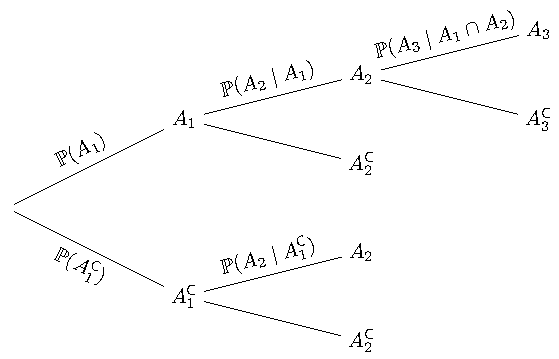
\includegraphics{./stoch_abbildungen/baum_1.pdf}
	\captionof{figure}{Darstellung eines Stufenexperiments}
\end{center}

\begin{satz}[ Wahrscheinlichkeitsmaß eines Stufenexperiments] \label{satz: 3_1_6_stufenexperiment}
	Gegeben seinen $n$ Ergebnisräume $\Omega_i = \menge{\omega_i (1), \dots, \omega_i (k)}, k \in \N \cup \menge{\infty}$ und es sei $\Omega = \Omega_1 \times \cdots \Omega_n$ der zugehörige Produktraum. Weiter seinen $\F_i$ $\sigma$-Algebren auf $\Omega_i$ und $\F = \bigotimes_{i=1}^n \F_i$ die Produkt-$\sigma$-Algebra auf $\Omega$. Setze $\omega = (\omega_1,\dots,\omega_n)$ und
	\begin{equation*}
	[\omega_1,\dots,\omega_m] \defeq \menge{\omega_1}\times \dots \times \menge{\omega_m} \times \Omega_{m+1} \times \cdots \times \Omega_{n} \qquad (m \leq n) 
	\end{equation*}
	und
	\begin{equation*}
		\P(\menge{\omega_m} \mid [\omega_1,\dots,\omega_{m-1}])
	\end{equation*}
	für die Wahrscheinlichkeit in der $m$-ten Stufe des Experiments $\omega_m$ zu beobachten, falls in den vorausgehenden Stufen $\omega_1,\dots,\omega_{m-1}$ beobachten wurden. Dann definiert
	\begin{equation*}
		\P(\menge{\omega}) \defeq \P(\menge{\omega_1}) \prod_{m=2}^{n}\P\brackets{\menge{\omega_m} \mid [\omega_1, \dots, \omega_{m-1}]}
	\end{equation*}
	ein Wahrscheinlichkeitsmaß auf $(\Omega, \F, \P)$.
\end{satz}
\begin{proof}
	Nachrechnen!
\end{proof}

\begin{beispiel}[\person{Polya}-Urne]
	Gegeben sei eine Urne mit $s$ schwarzen und $w$ weißen Kugeln. Bei jedem Zug wird die  gezogene Kugel zusammen mit $c \in \N_0 \cup \menge{-1}$ weiteren Kugeln derselben Farbe zurückgelegt.
	\begin{itemize}
		\item $c=0$: Urnenmodell mit Zurücklegen
		\item $c=-1$: Urnenmodell ohne Zurücklegen
	\end{itemize}
	Beide haben wir schon in Kapitel 2.2 gesehen. 
	Sei deshalb $c\in \N$ (Bsp. Modell für zwei konkurrierende Populationen). Ziehen wir $n$-mal, so haben wir ein $n$-Stufenexperiment mit 
	\begin{equation*}
		\Omega = \menge{0,1}^n \mit \text{ 0 = ``weiß'', 1 = ``schwarz''} \quad (\Omega_i = \menge{0,1})
	\end{equation*}
	Zudem gelten im ersten Schritt
	\begin{equation*}
		\P(\menge{0}) = \frac{w}{s+w} \und \P(\menge{1}) = \frac{s}{s+w}
	\end{equation*}
	sowie
	\begin{equation*}
		\P(\menge{\omega_m} \mid [\omega_1, \dots \omega_{m-1}]) = 
		\begin{cases}
		\frac{w+c \brackets{m-1 - \sum_{i=1}^{m-1}\omega_i}}{s+w+c(m-1)} & \omega_m = 0\\
		\frac{s + c\sum_{i=1}^{m-1}\omega_i}{s+w+c(m-1)} & \omega_m = 1
		\end{cases}
	\end{equation*}
	Mit \cref{satz: 3_1_6_stufenexperiment} folgt als Wahrscheinlichkeitsmaß auf $(\Omega, \pows(\Omega))$
	\begin{equation*}
	\begin{aligned}
		\P(\menge{(\omega_1, \dots, \omega_n)}) 
		&= \P(\menge{\omega_1}) \prod_{m=2}^n \P(\menge{\omega_m}\mid [\omega_1,\dots,\omega_{m-1}]) \\
		&= \frac{\prod_{i=0}^{l-1}(s+c * i) \, \prod_{j=0}^{n-l-1}(w + c * j)}{\prod_{i=0}^n (s+w+c * i)}
	\end{aligned}
	\end{equation*}
	mit $l=\sum_{i=1}^n \omega_i$. Definiere wir nun die Zufallsvariable
	\begin{equation*}
		\abb{S_n}{\Omega}{\N_0} \mit (\omega_1, \dots, \omega_n) \mapsto \sum_{i=1}^n \omega_i
	\end{equation*}
	welche die Anzahl der gezogenen schwarzen Kugeln modelliert, so folgt
	\begin{equation*}
		\P(S_n = l) = \binom{n}{l} \frac{\prod_{i=0}^{l-1}(s+c * i) \, \prod_{j=0}^{n-l-1}(w + c * j)}{\prod_{i=0}^n(s+w+c * i)}
	\end{equation*}
	Mittels $a \defeq \lfrac{s}{c}$ und $b \defeq \lfrac{w}{c}$ folgt
	\begin{equation*}
		\begin{aligned}
			\P(S_n = l) = \binom{n}{l} \frac{\prod_{i=0}^{l-1}(-a-i)\prod_{j=0}^{n-l-1}(-b-j)}{\prod_{i=0}^n (-a-b-i)} = \frac{\binom{-a}{l}\binom{-b}{n \cdot l}}{\binom{-a-b}{n}} \mit l \in \menge{0,\dots,n} 
		\end{aligned}
	\end{equation*}
	Dies ist die \begriff{\person{Polya}-Verteilung} auf $\menge{0,\dots,n}$ ($n \in \N$) mit Parametern $a,b > 0$.
\end{beispiel}

\begin{beispiel} \label{beispiel_3_1_8_multiplechoice}
	Ein Student beantwortet eine Multiple-Choice-Frage mit vier Antwortmöglichkeiten, eine davon ist richtig. Er kennt die richtige Antwort mit Wahrscheinlichkeit $\lfrac{2}{3}$. Wenn er die richtige Antwort kennt, so wählt er diese aus. Andernfalls wählt er zufällig (gleichverteilt) eine Antwort. Betrachten wir 
	\begin{equation*}
		W = \menge{\text{richtige Antwort gewusst}} \und 
		R = \menge{\text{Richtige Antwort gewählt}}
	\end{equation*}
	Dann gilt
	\begin{equation*}
		\P(W) = \frac{2}{3} \qquad \P(R \mid W) = 1 \qquad \P(R \mid W^\complement) = \frac{1}{4}
	\end{equation*}
	Angenommen der Student gibt die richtige Antwort. Mit welcher Wahrscheinlichkeit hat er diese gewusst? $\longrightarrow \enskip \P(W \mid R) = \text{ ?}$
\end{beispiel}

\begin{satz} \label{satz: 3_1_9_totaleW_bayes}
	Sei $(\Omega, \F, \P)$ ein Wahrscheinlichkeitsraum und $\Omega = \bigcup_{i \in I} B_i$ eine höchstens abzählbare Zerlegung in paarweise disjunkte Ereignisse $B_i \in \F$.
	\begin{enumerate}
		\item \textit{Satz von der totalen Wahrscheinlichkeit:} Für alle $A \in \F$ gilt
		\begin{align}
			\P(A) = \sum_{i\in I} \P(A\mid B_i) * \P(B_i) \label{eq: totaleWkeit}
		\end{align} 
		\item \textit{Satz von Bayes:} Für alle $A \in \F$ mit $\P(A) > 0$ und alle $k \in I$ gilt
		\begin{align}
			\P(B_k \mid A) = \frac{\P(A \mid B_k) * \P(B_k)}{\sum_{i\in I}\P(A\mid B_i) * \P(B_i)} \label{eq: bayes}
		\end{align}
	\end{enumerate}
\end{satz}

\begin{proof}
	Es gilt:
	\begin{equation*}
		\sum_{i\in I} \P(A\mid B_i) * \P(B_i) = \sum_{i\in I}\frac{\P(A \cap B_i)}{\P(B_i)} * \P(B_i) = \sum_{i\in I} \P(A \cap B_i) \overset{\sigma-Add.}{=} \P(A)
	\end{equation*}
	und
	\begin{equation*}
	\P(B_k \mid A) = \frac{\P(A \cap B_k)}{\P(A)} = \frac{\P(A \mid B_k) * \P(B_k)}{\P(A)}
	\end{equation*}
	also folgt (b) aus (a).
\end{proof}

\begin{beispiel}
	In der Situation von \cref{beispiel_3_1_8_multiplechoice} folgt mit \labelcref{eq: totaleWkeit}
	\begin{equation*}
	\begin{aligned}
		\P(R) 
		&= \P(R \mid W) * \P(W) + \P(R \mid W^\complement) * \P(W^\complement) \\
		&= 1 \cdot \frac{2}{3} + \frac{1}{4} * \frac{1}{3} = \frac{3}{4}
	\end{aligned}
	\end{equation*}
	und mit \labelcref{eq: bayes}
	\begin{equation*}
		\P(W \mid R) = \frac{\P(R \mid W) * \P(W)}{\P(R)} = \frac{1 * \frac{2}{3}}{\frac{3}{4}} = \frac{8}{9}
	\end{equation*}
	für die gesuchte Wahrscheinlichkeit.
	\begin{center}
		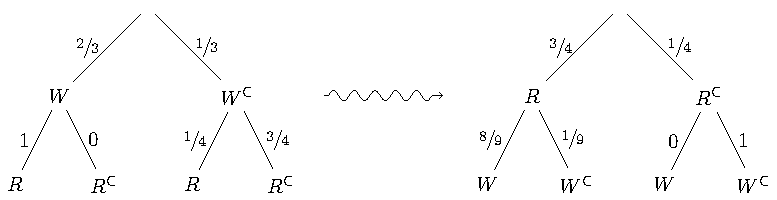
\includegraphics{./stoch_abbildungen/baum_2.pdf}
		\captionof{figure}{Bedingte Wahrscheinlichkeit im Baumdiagramm}
	\end{center}
\end{beispiel}
\section{Stochastische Unabhängigkeit} \label{sec: unabhaengigkeit}
In vielen Fällen besagt die Intuition über verschiedene Zufallsexperimente / Ereignisse, dass diese sich \textit{nicht} gegenseitig beeinflussen. Für solche $A,B \in \F$ mit $\P(A) > 0$ und $\P(B) > 0$ sollte gelten
\begin{equation*}
	\P(A\mid B) = \P(A) \quad \und \quad \P(B\mid A) = \P(B).
\end{equation*}

\begin{definition} \label{def: 3_2_11}
	Sei $(\Omega, \F, \P)$ Wahrscheinlichkeitsraum. Zwei Ereignisse $A,B \in \F$ heißt \begriff{(stochastisch) unabhängig} bezüglich $\P$, falls
	\begin{equation*}
		\P(A\cap B) = \P(A) * \P(B)
	\end{equation*}
	Wir schreiben auch $A \upmodels B$.
\end{definition}

\begin{beispiel}
	Wir betrachten wieder das Würfeln mit 2 fairen, sechsseitigen Würfeln. 
	\begin{equation*}
		\Omega = \menge{(i,j) \mid i,j \in\menge{1,\dots,n}} \qquad 
		\F = \pows\Omega \qquad 
		\P = \Uni(\Omega)
	\end{equation*}
	Betrachte
	\begin{equation*}
	\begin{aligned}
		A &\defeq \menge{(i,j) \in \Omega \colon i \text{ gerade}}\\
		B &\defeq \menge{(i,j) \in \Omega \colon j \leq 2}
	\end{aligned}
	\end{equation*}
	In diesem Fall, erwarten wir intuitiv die Unabhängigkeit von $A$ und $B$.
	In der Tat ist $\P(A) = \lfrac{1}{2}$, $\P(B) = \lfrac{1}{3}$ und $\P(A\cap B) = \lfrac{1}{6}$, womit $\P(A \cap B) = \P(A) * \P(B)$ erfüllt ist.
	Betrachte nun
	\begin{equation*}
	\begin{aligned}
		C &\defeq \menge{(i,j) \in \Omega \colon i + j = 7}\\
		D &\defeq \menge{(i,j) \in \Omega \colon i = 6}
	\end{aligned}
	\end{equation*}
	Dann gilt $\P(C) = \lfrac{1}{6}$ und $\P(D) = \lfrac{1}{6}$. Wegen $C \cap D = \menge{(6,1)}$ folgt
	\begin{equation*}
		\P(C\cap D) = \frac{1}{36} = \frac{1}{6} * \frac{1}{6} = \P(C) * \P(D)
	\end{equation*}
	$C$ und $D$ sind also \textit{stochastisch} unabhängig, obwohl eine kausale Abhängigkeit vorliegt.
\end{beispiel}

\begin{definition}
	Sei $(\Omega, \F, \P)$ ein Wahrscheinlichkeitsraum und $I \neq \emptyset$ eine endliche Indexmenge. Dann heißt die Familie $(A_i)_{i \in I}$ von Ereignissen in $\F$ \begriff{unabhängig} bezüglich $\P$, falls für alle $\emptyset \neq J \subseteq I$ gilt
	\begin{equation*}
		\P\brackets{\bigcap_{i \in J} A_i} = \prod_{i \in J} \P(A_i)
	\end{equation*}
	Offensichtlich impliziert die Unabhängigkeit einer Familie die paarweise Unabhängigkeit je zweier Familienmitglieder nach \cref{def: 3_2_11}. Umgekehrt gilt dies nicht.
\end{definition}

\begin{beispiel}[Abhängigkeit trotz paarweiser Unabhängigkeit]
	Wir betrachten ein zweifaches Bernoulliexperiment mit Erfolgswahrscheinlichkeit $\lfrac{1}{2}$, d.h.
	\begin{equation*}
		\Omega = \menge{0,1}^2 \qquad \F = \pows\Omega \qquad \P = \Uni(\Omega)
	\end{equation*}
	sowie
	\begin{equation*}
	\begin{aligned}
		A &= \menge{1} \times \menge{0,1} \qquad &&\text{(Münzwurf: erster Wurf ist Zahl)}\\
		B &= \menge{0,1} \times \menge{1} &&\text{(Münzwurf: zweiter Wurf ist Zahl)}\\
		C &= \menge{(0,0), (1,1)} &&\text{(beide Würfe haben selbes Ergebnis)}
	\end{aligned}
	\end{equation*}
	Dann gelten $\P(A) = \lfrac{1}{2} = \P(B) = \P(C)$ und
	\begin{equation*}
	\begin{aligned}
		\P(A\cap B) &= \P(\menge{(1,1)}) = \lfrac{1}{4} = \P(A) * \P(B)\\
		\P(A\cap C) &= \P(\menge{(1,1)}) = \lfrac{1}{4} = \P(A) * \P(C)\\
		\P(B\cap C) &= \P(\menge{(1,1)}) = \lfrac{1}{4} = \P(B) * \P(C)
	\end{aligned}
	\end{equation*}
	Daraus folgt also paarweise Unabhängigkeit. Jedoch ist
	\begin{equation*}
		\P(A \cap B \cap C) = \P(\menge{(1,1)}) = \frac{1}{4} \neq \P(A) * \P(B) * \P(C)
	\end{equation*}
	und $A,B,C$ sind \textit{nicht} stochastisch unabhängig.
\end{beispiel}

\begin{definition}[Unabhängige $\sigma$-Algebren] \label{3_15_def}
	Seien $(\Omega, \F,\P)$ ein Wahrscheinlichkeitsraum, $I \neq \emptyset$ eine Indexmenge und $(E_i, \Ecal_i)$ Messräume.
	\begin{enumerate}[leftmargin=*]
		\item Die Familie $\F_i \subset \F (i \in I)$, heißen \begriff{unabhängig}, wenn für die $\emptyset \neq J \subseteq I$ mit $\abs{J} < \infty$ gilt
		\begin{equation*}
			\P\brackets{\bigcap_{i \in J} A_i} = \prod_{i \in J} \P(A_i) \qquad \text{ für beliebige } A_i \in \F_i (i \in J)
		\end{equation*}
		\item Die Zufallsvariable $\abb{X_i}{(\Omega, \F)}{(E_i, \Ecal_i)} (i \in I)$, heißen \begriff{unabhängig}, wenn die $\sigma$-Algebren
		\begin{equation*}
			\sigma(X_i) = X^{-1}(\Ecal_i) = \menge{\menge{X_i \in F} \colon F \in \Ecal_i} \quad (i \in I)
		\end{equation*}
		unabhängig sind.
	\end{enumerate}
\end{definition}

\begin{lemma}[Zusammenhang der Definitionen]
	\label{3_16_lemma}
	Sei $(\Omega,\F,\P)$ ein Wahrscheinlichkeitsraum, $I \neq \emptyset$, $A_i \in \F_i$ für alle $i \in I$. 
	Die folgenden Aussagen sind äquivalent:
	\begin{enumerate}[nolistsep]
		\item Die Ereignisse $A_i$ ($i \in I$) sind unabhängig. 
		\item Die $\sigma$-Algebren $\sigma(A_i)$ ($i \in I$) sind unabhängig.
		\item Die Zufallsvariablen $\one_{A_i}$ ($i \in I$) sind unabhängig.
	\end{enumerate}
\end{lemma}
\begin{proof}
	Da die Unabhängigkeit über endliche Teilemengen definiert ist, können wir oBdA $I = \menge{1, \dots, n}$ annehmen. 
	\begin{itemize}[leftmargin=*, nolistsep]
		\item Da $\sigma(\one_{A_i}) = \sigma(A_i)$ folgt die Äquivalenz von (2) und (3) direkt aus \cref{3_15_def}.
		\item Zudem ist (2) $\to$ (1) klar.
		\item Für (1) $\to$ (2) genügt es zu zeigen, dass
		\begin{equation*}
			A_1, \dots, A_n \text{ unabhängig } \Rightarrow B_1, \dots, B_n \text{ unabhängig mit } B_i \in \menge{\emptyset, A_i, A_i^\complement, \Omega}
		\end{equation*}
		Rekursiv folgt dies bereits aus
		\begin{equation*}
			A_1,\dots, A_n \text{ unabhängig } \Rightarrow B_1, A_2, \dots, A_n \text{ unabhängig mit } B_1 \in \menge{\emptyset, A_1, A_1^\complement, \Omega}.
		\end{equation*}
		Für $B_1 \in \menge{\emptyset, A_1, \Omega}$ ist dies klar.\\
		Sei also $B_1 = A_1^\complement$ und $J \subseteq I$, $J \neq \emptyset$. Falls $1 \notin J$, ist nichts zu zeigen. Sei $1 \in J$, dann gilt mit $A = \bigcap_{i\in J, i \neq 1} A_i$ sicherlich
		\begin{equation*}
			\begin{aligned}
				\P\brackets{A_1^\complement \cap A} 
				&= \P(A \setminus (A_1 \cap A))\\
				&= \P(A) - \P(A_1 \cap A)\\
				&= \prod_{i\in J \setminus \menge{1}} \P(A_i) - \prod_{i\in J}(A_i) \\
				&= (1- \P(A_1))\prod_{i\in J\setminus \menge{1}} \P(A_i)\\
				&= \P\brackets{A_1^\complement} \prod_{i\in J \setminus \menge{1}} \P(A_i)
			\end{aligned}
		\end{equation*}
	\end{itemize}
\end{proof}

Insbesondere zeigt \cref{3_16_lemma}, dass wir in einer Familie unabhängiger Ereignisse beliebig viele Ereignisse durch ihr Komplement, $\emptyset$ oder $\Omega$ ersetzen können ohne die Unabhängigkeit zu verlieren.

\begin{satz}
	\label{3_17_satz}
	Sei $(\Omega, \F, \P)$ Wahrscheinlichkeitsraum und $\F_i \subseteq \F, i \in I$, seien $\cap$-stabile Familien von Ereignissen. Dann gilt
	\begin{equation*}
		\F_i (i \in I) \text{ unabhängig } \equivalent \sigma(\F_i) (i \in I) \text{ unabhängig}. 
	\end{equation*}
\end{satz}

\begin{proof}
	oBdA sei $I = \menge{1, \dots, n}$ und $\Omega \in \F_i, i \in I$.
	\begin{proof-equivalence}[leftmargin=*, nolistsep]
		\rueckrichtung trivial, da $\F_i \subseteq \sigma(\F_i)$ und das Weglassen von Mengen erlaubt ist.
		\hinrichtung zeigen wir rekursiv
		\begin{enumerate}[label=(\roman*), nolistsep]
			\item Wähle $F_i \in \F_i, i = 2, \dots,n$ und definiere für $F \in \sigma(\F_i)$ die endlichen Maße
			\begin{equation*}
				\mu(F) = \P\brackets{ F \cap F_2 \cap \cdots \cap F_n} \und \nu(F) = \P(F) \, \P(F_2) \, \dots \, \P(F_n)
			\end{equation*}
			\item Da die Familien $\F_i$ unabhängig sind, gilt
			$\mu\mid_{\F_1} = \nu\mid_{\F_1}$.
			Nach dem Eindeutigkeitssatz für Maße (\cref{satz: 1.9_eindeutigkeitssatz}) folgt $\mu\mid_{\sigma(\F_1)} = \nu\mid_{\sigma(\F_1)}$ also
			\begin{equation*}
				\P\brackets{ F \cap F_2 \cap \cdots \cap F_n} = \P(F) \P(F_2) \dots \P(F_n)
			\end{equation*}
			für alle $F \in \sigma(\F_i)$ und $F_i \in \F_i, i = 1, \dots, n$. Da $\Omega \in \F_i$ für alle $i$ gilt die erhaltene Produktformel auf für alle Teilemengen $J \subseteq I$.\\
			Also sind $\sigma(\F_1), \F_2, \dots, \F_n$ unabhängig.
			\item Wiederholtes Anwenden von (i) und (ii) liefert den Satz.
		\end{enumerate}
	\end{proof-equivalence}
\end{proof}
%
Mit \cref{3_17_satz} folgen:

\begin{korollar}	\label{3_18_kor}
	Sei $(\Omega,\F,\P)$ ein Wahrscheinlichkeitsraum und $\F_{i,j} \subseteq \F$ mit $1 \le i \le n, 1 \le j \le m(i)$ unabhängige, $\cap$-stabile Familien.
	Dann sind auch
	\begin{equation*}
		\G_i = \sigma(\F_{i,1}, \dots , \F_{i,m(i)}), \quad 1 \le i \le n
	\end{equation*}
	unabhängig.
\end{korollar}
\begin{proof}
	oBdA sei $\Omega \in \F_{i,j} \enskip \forall i,j$, da $\Omega$ die Unabhängigkeit nach \cref{3_16_lemma} nicht zerstört.
	Dann sind die Familien 
	\begin{equation*}
		\F_i^\cap \defeq \menge{F_{i,1} \cap \cdots \cap F_{i,m(i)} : F_{i,j} \in \F_{i,j}, 1 \le j \le m(i)} \enskip (1 \le i \le n)
	\end{equation*}
	$\cap$-stabil, unabhängig und es gilt $\F_{i,1}, \dots , \F_{i,m(i)} \subseteq \F_i^\cap$ (vgl. Hausaufgabe). Nach \cref{3_17_satz} sind auch $\sigma(\F_i^\cap)$ unabhängig. Damit folgt die Behauptung, da aus 
	\begin{equation*}
		\F_{i,1}, \dots , \F_{i,m(i)} \subseteq \F_i^\cap \subseteq \sigma(\F_{i,1}, \dots , \F_{i,m(i)}) = \G_i
	\end{equation*} unter Anwendung des Erzeugenden-Operators $\G_i = \sigma(\F_{i,1}, \dots , \F_{i,m(i)}) \subseteq \sigma(\F_i^\cap) \subseteq \G_i$ folgt, d.h. $\sigma(\F_i^\cap) = \G_i$.
\end{proof}

\begin{korollar} \label{3_19_korollar}
	Sei $(\Omega,\F,\P)$ ein Wahrscheinlichkeitsraum und $\abb{X_{i,j}}{\Omega}{E}$ ($1 \le i \le n, 1 \le j \le m(i)$)
	unabhängige Zufallsvariablen. Zudem seinen $\abb{f_i}{E^{m(i)}}{\R}$ messbar. Dann sind auch die Zufallsvariablen $f_i(X_{i,1}, \dots, X_{i,m(i)})$ mit $1 \le i \le n$ unabhängig.
\end{korollar}
\begin{proof}
	Setze $\F_{i,j} = \sigma(X_{i,j})$ und $\G_i = \sigma(\F_{i,1} , \dots , \F_{i,m(i)})$. Dann sind nach \cref{3_18_kor} die $\G_i$ ($i = 1, \dots , n)$ unabhängig. Zudem ist $Y_i \defeq f_i(X_{i,1}, \dots , X_{i,m(i)})$ $\G_i$-messbar, also $\sigma(Y_i) \subseteq \G_i$. Damit erben die $Y_i$ die Unabhängigkeit der $\G_i$.
\end{proof}

\begin{beispiel}
	Seien $X_1, \dots, X_n$ unabhängige, reelle Zufallsvariablen. Dann sind auch
	\begin{equation*}
	Y_1 = X_1, Y_2 = X_2 + \cdots + X_n
	\end{equation*}
	unabhängig.
\end{beispiel}

\begin{satz}[Unabhängigkeit von Zufallsvariablen]
	\label{3_21_satz}
	Seien $(\Omega, \F, \P)$ ein Wahrscheinlichkeitsraum und $\abb{X_1, \dots, X_n}{(\Omega,\F)}{(E, \Ecal)}$ Zufallsvariablen. Dann sind äquivalent:
	\begin{enumerate}[label=(\arabic*), nolistsep]
		\item $X_1 , \dots , X_n$ sind unabhängig.
		\item $\P(X_1 \in A_1 , \dots , X_n \in A_n) = \prod_{i=1}^n \P(X_i \in A_i) \quad \forall A_1, \dots , A_n \in \Ecal$
		\item Die gemeinsame Verteilung der $X_i$ entspricht dem Produktmaß der einzelnen Verteilungen
		\begin{equation*}
			\P_{X_1 , \dots , X_n} = \P_{X_1} \otimes \dots \otimes \P_{X_n}
		\end{equation*}
	\end{enumerate}
\end{satz}
\begin{proof}
	per Ringschluss 
	\begin{description}[nolistsep]
		\item [(1 $\boldsymbol{\Rightarrow}$ 2)] Seien $A_1, \dots, A_n \in \Ecal$ beliebig. Dann gilt per Definition
		\begin{equation*}
			\begin{aligned}
				\P_{X_1 , \dots , X_n}(A_1 \times \dots A_n) 
				&= \P(X_1 in A_1, \dots , X_n \in A_n) \\
				&= \P\brackets{\bigcap_{i=1}^n \menge{X_i \in A_i}} \\
				&= \prod_{i=1}^n \P(X_i \in A_i) \\
				&= \prod_{i=1}^n \P_{X_i}(A_i) \\
				&= \brackets{\bigotimes_{i=1}^n \P_{X_i}} \brackets{A_1 \times \dots \times A_n}
			\end{aligned}
		\end{equation*}
		\item [(2 $\boldsymbol{\Rightarrow}$ 3)] Aus der obigen Gleichung sehen wir, dass (2) bereits (3) impliziert für alle Rechtecke $A_1 \times \dots \times A_n$. Da die Familie der Rechtecke $\cap$-stabil ist und $\Ecal^{\otimes n}$ erzeugt, folgt die Aussage aus dem Eindeutigkeitssatz für Maße.
		\item [(3 $\boldsymbol{\Rightarrow}$ 1)] Es sei $J \subseteq \menge{1, \dots, n}$ und 
		\begin{equation*}
			A_i \defeq \begin{cases}
			\text{beliebig in } \Ecal & \text{falls } i \in J \\
			E & \text{falls } i \notin J
			\end{cases}
		\end{equation*}
		Dann ist
		\begin{equation*}
			\begin{aligned}
			\P(X_i \in A_i : i \in  J) 
			&= \P(X_i \in A_i : i = 1 , \dots , n) \\
			&= \prod_{i=1}^n \P(X_i \in A_i) \\
			&= \prod_{i \in J} \P(X_i \in A_i)
			\end{aligned}
		\end{equation*}
	\end{description}
\end{proof}

\begin{beispiel}
	Im Urnenmodell mit Zurücklegen hat der Vektor $X = (X_1, \dots , X_n)$ mit $X_i$ = Farbe im $i$-ten Zug als Zähldichte die Produktdichte der $X_i$. $X_1 , \dots , X_n$ sind also unabhängig.
\end{beispiel}
\subsection{Konstruktion unabhängiger Zufallsvariablen}
\cref{chapter_1_grundbegriffe}: Zu beliebiger Wahrscheinlichkeitsverteilung $\P_X$ existiert ein Wahrscheinlichkeitsraum mit Zufallsvariable $X$ auf diesem Wahrscheinlichkeitsraum, so dass $X \sim \P_X$.

\begin{enumerate}[leftmargin=*, nolistsep]
	\item Seien $\P_{X_1}, \P_{X_2}$ Wahrscheinlichkeitsverteilungen auf $(E, \Ecal)$. Gibt es einen Wahrscheinlichkeitsraum $(\Omega, \F, \P)$ und Zufallsvariablen $X_1, X_2$ unabhängig, so dass $X_i \sim \P_{X_i}$?
	\item Wie kann ich beliebig (unendlich) viele unabhängige Zufallsvariablen konstruieren?
\end{enumerate}

Wir beginnen mit Schritt (1):

Konstruiere zwei Wahrscheinlichkeitsräume $(\Omega_i, \F_i, \P_i)$ ($i = 1,2$) und Zufallsvariablen $X_1, X_2$ mit $X_i \sim \P_{X_i}$. Auf dem Produktraum
\begin{equation*}
	\Omega \defeq \Omega_1 \times \Omega_2 \quad \F \defeq \F_1 \otimes \F_2 \quad \P = \P_1 \otimes \P_2
\end{equation*}
definieren wir
\begin{equation*}
\begin{aligned}
	X'_1 \colon \Omega_1 \times \Omega_2 \to E : &(\omega_1, \omega_2) \mapsto X_1(\omega_1) \\
	X'_2 \colon \Omega_1 \times \Omega_2 \to E : &(\omega_1, \omega_2) \mapsto X_2(\omega_2)
\end{aligned}
\end{equation*}
Dann gilt für beliebige Ereignisse: $F_1, F_2 \in \Ecal$
\begin{equation*}
	\underbrace{\menge{X'_1 \in F_1} \cap \menge{X'_2 \in F_2}}_{\supseteq \Omega = \Omega_1 \times \Omega_2} = \underbrace{\menge{X_1 \in F_1}}_{\supseteq \Omega_1} \times \underbrace{\menge{X_2 \in F_2}}_{\supseteq \Omega_2} \in \F_1 \times \F_2
\end{equation*}
und damit folgt die Messbarkeit der Abbildungen $X'_1, X'_2$, d.h. $X'_1, X'_2$ sind Zufallsvariablen auf $(\Omega, \F)$. Zudem gilt
\begin{equation*}
\begin{aligned}
	\P(X'_1 \in F_1, X'_2 \in F_2)
	&= \P_1 \otimes \P_2 \brackets{\menge{X_1 \in F_1} \times \set{X_2 \in F_2}} \\
	&= \P_1 (X_1 \in F_1) \P_2(X_2 \in F_2)
\end{aligned}
\end{equation*}
also $\P(X'_i \in F_i) = \P_i (X'_i \in F_i)$ sowie nach \cref{3_21_satz} $X'_1 \upmodels X'_2$.

Wenn $(\Omega_2, \F_1, \P_1) = (\Omega_2, \F_2, \P_2)$, so liefert die obige Konstruktion zwei unabhängige Zufallsvariablen auf einem Wahrscheinlichkeitsraum. Andernfalls können wir auf den Produktraum ausweichen und $X'_i$ anstelle von $X_i$ betrachten. Die obige Konstruktion lässt sich direkt auf \textit{endlich} viele Zufallsvariablen übertragen.

Betrachten wir nun den Fall (2). Wir benötigen dafür den folgenden Satz.

\begin{satz}[Satz von \person{Kolmogorov}]
	\label{3_23_satz_kolmogorov}
	Sei $I$ eine beliebige Indexmenge und $(\Omega_i, \F_i, \P_i)$ ($i \in I$) Wahrscheinlichkeitsräume. Setze
	\begin{equation*}
		\begin{aligned}
		\Omega_I &\defeq \bigtimes_{i \in I} \Omega_i = \menge{\omega : I \to \bigcup_{i \in I} \Omega_i, \omega_i \in \Omega_i, i \in I}\\
		\F_I &:= \sigma( \pi^{-1} ( \F_i) : i \in I)
		\end{aligned}
	\end{equation*}
	wobei $\abb{\pi_i}{\Omega_I}{\Omega_i}$ mit $\omega \mapsto \omega_i$ die Projektionsabbildung ist. Dann existiert auf $(\Omega_I, \F_I)$ genau ein Wahrscheinlichkeitsmaß $\P_I$, sodass für alle $H \subseteq I$ mit $0 \le \abs{H} < \infty$ gilt
	\begin{equation*}
		\pi_H ( \P_I) = \bigotimes_{i \in H} \P_i,
	\end{equation*}
	wobei $\abb{\pi_i}{\Omega_I}{\Omega_H}$ wiederum die Projektionsabbildung.
\end{satz}
\begin{proof}
	$\nearrow$ Schilling: Maß und Integral, Satz 17.4.
\end{proof}

Sind auf den Wahrscheinlichkeitsräumen $(\Omega_i , \F_i , \P_i)$ ($i \in I$), nun Zufallsvariablen $\abb{X_i}{\Omega_i}{E}$ gegeben, so definieren wir wie im Satz von Kolmogorov (\cref{3_23_satz_kolmogorov})
\begin{equation*}
	(\Omega, \F, \P) \defeq \brackets{\Omega_I, \F_I, \P_I = \bigotimes_{i \in I} \P_i} \mit \omega = (\omega_i)_{i \in I}
\end{equation*}
und wie im endlichen Fall
\begin{equation*}
	\abb{X_i'}{\Omega}{E} \mit X_i'(\omega) = X_i(\omega_i)
\end{equation*}
definieren. Da die Unabhängigkeit der Zufallsvariablen über endliche Teilfamilien definiert ist, folgt diese wie im endlichen Fall. 
\section{Faltungen}

Seien $X,Y$ zwei reelle unabhängige Zufallsvariablen mit $X \sim \P_X$ und $Y \sim \P_Y$. Dann hat $(X,Y)$ die Verteilung $\P_X \otimes \P_Y$ auf $\R^2$. Anderseits ist auch $X+Y$ eine reelle Zufallsvariable, denn $X + Y = A(X,Y)$ für $\abb{A}{\R^2}{\R}$ mit $(x,y) \mapsto x+y$. $A$ ist stetig, also messbar. Die Verteilung von $X+Y$ ist dann $\brackets{\P_X \otimes \P_Y} \circ A^{-1}$.

\begin{definition}
	Seien $\P_1$ und $\P_2$ Wahrscheinlichkeitsmaße auf $(\Rn, \borel{\Rn})$. Das durch 
	\begin{equation*}
		\P_1 \ast \P_2 (F) \defeq \iint \one_F(x+y) \P_1(\mathrm{d}x) \P_2(\mathrm{d}y)
	\end{equation*}
	definierte Wahrscheinlichkeitsmaß $\P_1 \ast \P_2 = (\P_1 \otimes \P_2) \circ A^{-1}$ auf $(\Rn, \borel{\Rn})$ heißt \begriff{Faltung} von $\P_1$ und $\P_2$.
\end{definition}

\begin{satz} \label{3_25_satz}
	Seien $\abb{X,Y}{\Omega}{\Rn}$ unabhängige Zufallsvariablen mit Verteilungen $\P_X$ bzw. $\P_Y$. Dann ist 
	\begin{equation*}
		\P_{X+Y} = \P_X \ast \P_Y
	\end{equation*}
	die Verteilung von $X+Y$.
\end{satz}
\begin{proof}
	siehe Herleitung Faltung oben
\end{proof}

Faltungen von Wahrscheinlichkeitsmaßen mit Dichten besitzen wiederum eine Dichte.

\begin{proposition}
	Seien $\P_1$ und $\P_2$ Wahrscheinlichekeitsmaße auf $(\R, \borel{\R})$.
	\begin{enumerate}[leftmargin=*, nolistsep]
		\item \textbf{diskreter Fall:} Sind $\P_1$ und $\P_2$ de facto Wahrscheinlichkeitsmaße auf $(\Z, \pows{\Z})$ mit Zähldichten $\rho_1$ und $\rho_2$, dann ist $\P_1 \ast \P_2$ ein Wahrscheinlichkeitsmaß auf $(\Z, \pows{\Z})$ mit Zähldichte
		\begin{equation*}
			\rho_1 \ast \rho_2 (k) = \sum_{\ell \in \Z} \rho_1(\ell) \rho_2(k-\ell) \quad (k \in \Z)
		\end{equation*}
		\item \textbf{stetiger Fall:} Wenn $\P_1$ und $\P_2$ Dichtefunktionen $\rho_1$ und $\rho_2$ besitzen, dann besitzt $\P_1 \ast \P_2$ die Dichtefunktion
		\begin{equation*}
			\rho_1 \ast \rho_2 (x) \defeq \int_\R \rho_1(y) \rho_2(x-y) \dy \quad (x \in \R)
		\end{equation*}
	\end{enumerate}
\end{proposition}
\begin{proof}
	\begin{description}
		\item[Diskreter Fall:] Sei $k \in \Z$.
		\begin{equation*}
			(\P_1 \otimes \P_2) (A = k) = \sum_{\ell_1,\ell_2 \in \Z ; \ell_1 + \ell_2 = k} \rho(\ell_1)\rho(\ell_2) = \sum_{\ell,k \in \Z} \rho_1(\ell) \rho_2(k-\ell) = \rho_1 \ast \rho_2 (k)
		\end{equation*}
		\item[Stetiger Fall:] Sei $c \in \R$.
		\begin{equation*}
			\begin{aligned}
			\P_1 \ast \P_2 ((-\infty , c]) 
			&= (\P_1 \otimes \P_2)(A \le c) \\
			&= \int_\R \int_\R \one_{(\infty,c]}(x+y) \rho_1(x) \rho_2(y) \dx \dy \\
			\overset{y = z - x}&{=} \int_\R \int_\R \one_{(\infty,c]}(z) \rho_1(x) \rho_2(z-x) \dx \dz \\
			&= \int_{-\infty}^c \underbrace{\int_\R \rho_1(x) \rho_2(z-x) \dx}_{\rho_1 \ast \rho_2 (z)} \dz
			\end{aligned}
		\end{equation*}
	\end{description}
\end{proof}

\begin{beispiel}
	Seien $X \sim \Poisson(\lambda)$ und $Y \sim \Poisson(\mu)$ zwei unabhängige reelle Zufallsvariablen (mit Werten in $\N_0$). Dann ist $X+Y$ eine Zufallsvariable mit Werten in $\N_0$ und Zähldichte
	\begin{equation*}
		\begin{aligned}
		\P(X+Y = k) &= \sum_{\ell \in \Z} \P(X=\ell) * \P(Y=k - \ell) \\
		&= \sum_{\ell = 0}^k \frac{\lambda^\ell}{\ell !} e^{-\lambda} * \frac{\mu^{k-\ell}}{(k-\ell)!} e^{-\mu}
		= e^{-(\lambda+\mu)} \frac{1}{k!} \sum_{\ell = 0}^k \binom{k}{\ell} \lambda^\ell \mu^{k-\ell} \\
		&= e^{-(\lambda + \mu)} \frac{1}{k!} (\lambda + \mu)^k
		\end{aligned}
	\end{equation*}
	sodass $X+Y \sim \Poisson(\lambda + \mu)$, d.h. der Typ der Verteilung ist bei der Faltung erhalten geblieben. Das ist aber nicht immer der Fall.
\end{beispiel}

\begin{beispiel}
	Seien $X,Y \sim \Uni([0,1])$ zwei unabhängige Zufallsvariablen mit Dichten $\rho(x) = \one_{[0,1]}(x)$. Dann ist $X+Y$ eine Zufallsvariable mit Werten in $[0,2]$ und Dichte 
	\begin{equation*}
		\begin{aligned}
		\rho \ast \rho (x) 
		&= \int_{\R} \rho(y) \rho(y-x) \dy 
		= \int_{1 \land x} \one_{[0,1]}(y) \one_{[0,1]}(y-x) \dy 
		= \int_{1 \lor (x-1)} \dy \\
		&= \begin{cases}
			x & 0 \le x \le 1 \\
			2-x & 1 \le x \le 2 \\
			0 & \text{sonst}
		\end{cases}
		\end{aligned}
	\end{equation*}
	
	\begin{center}
		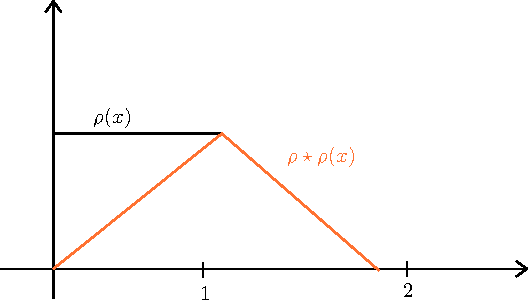
\includegraphics[width=.45\textwidth]{./stoch_abbildungen/faltung_dichte.pdf}
		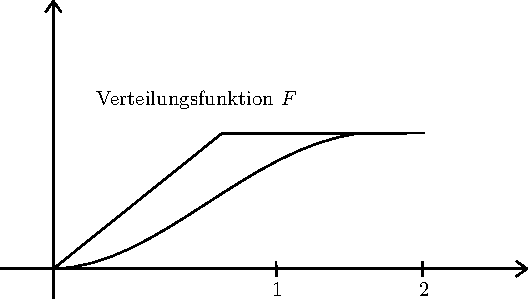
\includegraphics[width=.45\textwidth]{./stoch_abbildungen/faltung_verteilungsfunktion.pdf}
	\end{center}
	
\end{beispiel}

\chapter{Weitere Standardmodelle: Stetige Verteilungen}
\label{chapter_4_stetigeVerteilungen}
\section{Stetige Gleichverteilung}

\begin{*erinnerung}
	$\Omega \subset \Rn$ Borel-messbar mit Lebesgue-Volumen $0 < \lambda(\Omega) < \infty$. Wahrscheinlichkeitsmaß ist $(\Omega, \borel(\Omega))$ mit Dichte
	\begin{equation*}
		\rho(x) = \frac{1}{\lambda(\Omega)}
	\end{equation*}
	heißt stetige Gleichverteilung auf $\Omega$, notiert mit $\Uni(\Omega)$.
\end{*erinnerung}

Für alle $A \in \borel\Omega$ gilt:
\begin{equation*}
	\P(A) = \int_{A} \rho(x) \dx = \frac{\lambda(A)}{\lambda(\Omega)}.
\end{equation*}
Meist verwenden wir $\Uni([a,b])$ für $a < b$ (Gleichverteilung auf Intervall) mit \begin{equation*}
	\rho(x) = \frac{1}{(b-a)} \mit a \le x \le b
\end{equation*} 
und Verteilungsfunktion
\begin{equation*}
	F(x) = 
	\begin{cases}
	0 & x < a\\
	\int_{a}^{x} \frac{1}{b-a} \dy = \frac{x-a}{b-a} & a \le x \le b\\
	1 & x >b.
	\end{cases}
\end{equation*}
\section{Wartezeitverteilungen}

\subsection{Negative Binomialverteilung}

Wir wiederholen ein Bernoulliexperiment mit Erfolgswahrscheinlichkeit $p \in [0,1]$ unendlich oft. Gesucht ist die Anzahl der Misserfolge bis zum $r$-ten Erfolg ($r \in \N$). Ein passender Ergebnisraum ist $\Omega = \N_0$. Für Modellierung ist es jedoch leichter in jedem Versuch erfolgt (``1'') oder Misserfolg (``0'') festzuhalten und mit dem unendlichen Produktmaß des Bernoullimaßes auf $\menge{0,1}^{\N}$ zu arbeiten. 

Als Zufallsvariable wählen wir
\begin{equation*}
	\abb{X_r}{\menge{0,1}^\N}{\Omega}
\end{equation*}
welche die Anzahl der Misserfolge bis zum $r$-ten Erfolg darstellt. Setze
\begin{equation*}
	X_r(\omega) = \min\menge{k : \sum_{i=1}^{k} \omega_i = r} - r
\end{equation*}
Dann ist
\begin{equation}
	\P(X_r = k) = \sum_{\omega \in \menge{0,1}^\N, X_r(\omega) = k} \prod_{i=1}^{\infty} \rho(\omega_i) \tag{$\star$} \label{eq_negbin1}
\end{equation}
mit $\rho(0) = 1-p$ und $\rho(1) = p$ (Zähldichte der Binomialverteilung), also
\begin{equation*}
	\P(X_r = k) = \binom{r+k-1}{k} (1-p)^k p^r \quad (k \in \N)
\end{equation*}

\begin{*anmerkung}
	Alternativ kann \cref{eq_negbin1} auch durch
	\begin{equation*}
		\P(X_r = k) = \sum_{\omega \in \menge{0,1}^{r+k}, X_r(\omega) = k} \prod_{i=1}^{r+k} \rho(\omega_i)
	\end{equation*}
	ersetzt werden.
\end{*anmerkung}

\begin{definition}[negative Binomialverteilung]
	\label{4_1_defintion}
	Sei $p \in[0,1]$ und $r \in \N$, dann heißt die Verteilung auf $\N_0$ mit Zähldichte
	\begin{equation*}
		\rho(k) = \binom{r+k-1}{k} (1-p)^k p^r 
	\end{equation*}
	die \begriff{negative Binomialverteilung} mit Parametern $(r,p)$. Schreibe $\negBin(r,p)$. Im Fall $r = 1$ nennen wir die Verteilung mit Zähldichte
	\begin{equation*}
		\rho(k) = p (1-p)^k \quad (k \in \N_0)
	\end{equation*}
	\begriff{geometrische Verteilung} mit Parameter $p$. Schreibe $\Geom(p)$.
\end{definition}


\subsection{Exponential- und Gammaverteilung}

\begin{description}
	\item[Ziel:] Modelliere die Wartezeit auf $r$ Ereignisse in kontinuierlicher Zeit
	\item[Wähle:] $(\Omega, \F) = (\R_+, \borel(\R_+))$
	\item[Annahmen:] ~
	\begin{itemize}
		\item Jedes Ereignis geschieht zu einer zufälligen Zeit.
		\item Die Anzahl der Ereignisse bis zur Zeit $t$ sei $\Poisson(\lambda t)$ verteilt.
	\end{itemize}
\end{description}

Die zweite Annahme macht Sinn, denn
\begin{itemize}
	\item Poissonverteilung ist Modell für Anzahl seltener Ereignisse
	\item Nach Beispiel 3.26 gilt $\Poisson(\lambda t) \ast \Poisson(\lambda s) = \Poisson(\lambda(t+s))$. 
	Die Linearität des Parameters entspricht also einer Stationaritätsvorrausetzung -- Modelliert $X \sim \Poisson(\lambda t)$ die Ereignisse in $(0,t]$ und $Y \sim \Poisson(\lambda s)$ die Ereignisse in $(t,t+s]$, so modelliert $X+Y \sim \Poisson(\lambda (t+s))$ die Ereignisse in $(0,t+s]$.
\end{itemize}

Unter diesen Annahmen folgt für die Wahrscheinlichkeit in $(0,t]$ mindestens $r$ Ereignisse zu beobachten
\begin{equation*}
	\P ((0,t)) = 1-\sum_{k=0}^{r-1} \underbrace{e^{-\lambda t} \frac{(\lambda t)^k}{k!}}_{\text{Zähldichte } \Poisson(\lambda t)\text{ in } k}
\end{equation*}
Wegen
\begin{equation*}
\begin{aligned}
	\ableitung{t} \brackets{1- \sum_{k=0}^{r-1} e^{-\lambda t} \frac{(\lambda t)^k}{k!}}
	&= - (-\lambda) e^{-\lambda t} \sum_{k=0}^{r-1} \frac{(\lambda t)^k}{k!} - e^{-\lambda t} \sum_{k=1}^{r-1} \frac{\lambda^k t^{k-1}}{(k-1)!}  \\
	&= e^{-\lambda t} \left( \sum_{k=0}^{r-1} \frac{\lambda^{k+1} t^k}{k!} - \sum_{k=0}^{r-2} \frac{\lambda^{k+1} t^k}{k!} \right) \\
	&= e^{-\lambda t} \frac{\lambda^r t^{r-1}}{(r-1)!} 
\end{aligned}
\end{equation*}
gilt
\begin{equation*}
	\P((0,t)) = \int_{0}^t e^{-\lambda x} \frac{\lambda^r x^{r-1}}{(r-1)!} \dx
\end{equation*}

Wir definieren allgemeiner:
\begin{definition}[Gammaverteilung, Gammafunktion]
	\label{4_2_definition}
	Seien $\lambda > 0$ und $r>0$. Dann heißt die Verteilung auf $(\R_+, \borel{\R_+})$ mit Dichte
	\begin{equation*}
		f(x) = \frac{\lambda^r}{\Gamma(r)} x^{r-1} e^{-\lambda x} \quad \mit \quad 
		\Gamma(r) = \int_{0}^{\infty} y^{r-1}e^{-y} \dy \quad (r>0)
	\end{equation*}
	\begriff{Gammaverteilung} mit Parametern $\lambda,r$. Schreibe $\GammaDist(\lambda,r)$.
\end{definition}

Insbesondere ist $\GammaDist(\lambda,1)$ gerade die \begriff{Exponentialverteilung} $\Exp(\lambda)$ (vgl. \cref{beispiel: 1_1.7_exponentialverteilung}).

\begin{*anmerkung}
	Die Funktion $\Gamma$ in \cref{4_2_definition} wird auch als Gamma-Funktion bezeichnet.
\end{*anmerkung}

Die Gammaverteilung ist \begriff{reproduktiv}: Die Wartezeit auf $r+s$ Ereignisse entspricht der Wartezeit auf $r$ Ereignisse + $s$ (weitere) Ereignisse:
\begin{lemma}
	\label{4_3_lemma}
	Seien $X \sim \GammaDist(\lambda,r), Y \sim \GammaDist(\lambda,s)$ unabhängig. Dann gilt 
	\begin{equation*}
		X+Y \sim \GammaDist(\lambda,r+s)
	\end{equation*}
\end{lemma}
\begin{proof}
	Hier nur für $r,s \in \N$, allgemein später mit momenterzeugenden Funktionen. 
	Seien $\rho_X$, $\rho_Y$ Dichten von $X$,$Y$. Nach \cref{3_25_satz} folgt
\begin{align*}
	\rho_{X+Y}(x) 
	&= (\rho_X \ast \rho_Y) (x) 
	= \int_{\R} \rho_X(y)\rho_Y(x-y) \dy  \\
	&= \int_0^x \frac{\lambda^r}{\Gamma(r)} y^{r-1} e^{-\lambda y} \frac{\lambda^s}{\Gamma(s)} (x-y)^{s-1} e^{-\lambda (x-y)} \dy  \\
	&= \frac{\lambda^{r+s}}{\Gamma(r)\Gamma(s)} e^{-\lambda x} \int_0^x y^{r-1} (x-y)^{s-1} \dy  \\
	\overset{\text{P.I.}}&{=} \frac{\lambda^{r+s}}{\Gamma(r)\Gamma(s)} e^{-\lambda x} \brackets{\underbrace{\left[\frac{1}{r} y^r (x-y)^{s-1}\right]_{y=0}^x}_{=0} + \frac{s-1}{r} \int_0^x y^r (x-y)^{s-2} \dy }  \\
	\overset{\text{Induktion}}&{=} \frac{\lambda^{r+s}}{\Gamma(r)\Gamma(r)} e^{-\lambda x} \frac{\Gamma(r)\Gamma(s)}{\Gamma(r+s)} = \frac{\lambda^{r+s}}{\Gamma(r+s)} e^{-\lambda x}
\end{align*}
\end{proof}

Exponentialverteilungen sind zudem \begriff{gedächtnislos}:
\begin{lemma}[Gedächtnislosigkeit der Exponentialverteilung]
	\label{4_4_lemma}
	Sei $X \sim \Exp(\lambda)$. Dann gilt
	\begin{equation*}
		\P(X>t) = \P(X > t+s \mid X > s) \quad (t,s \ge 0) \tag{$\star$}\label{4_4_eq:gedaechtnislos}
	\end{equation*}
\end{lemma}
\begin{proof}
	\begin{align*}
		\P(X > t+s \mid X \ge s) &= \frac{\P(X > t+s, X > s)}{\P(X > s)} \\
		&= \frac{\P(X > t+s)}{\P(X > s)} \\
		&= \frac{e^{-\lambda(t+s)}}{e^{-\lambda t}} = e^{-\lambda t} = \P(X> t)
	\end{align*}
\end{proof}

\begin{beispiel}
	\label{4_5_beispiel}
	Eine Studentin wartet morgens eine $\Exp(\sfrac{1}{5})$ verteilte Zeit $X$ auf den Bus zur Uni. Die Wahrscheinlichkeit einer Wartezeit $\ge 5$ Minuten beträgt
	\begin{equation*}
		\P(X \ge 5) = e^{-\frac{1}{5} * 5} = e^{-1} \approx 0,37
	\end{equation*}
	An einem kalten, stürmischen Frühlingstag hat die Studentin bereits 10~Minuten gewartet. Die Wahrscheinlichkeit mindestens fünf weitere Minuten zu warten ist
	\begin{equation*}
		\P(X\ge 15 \mid X \ge 10) = \P(X \ge 5) = e^{-1} \approx 0,37
	\end{equation*}
\end{beispiel}

\begin{*bemerkung}
	Man kann sogar zeigen, dass die Exponentialverteilung die einzige absolutstetige Verteilung mit der Eigenschaft \labelcref{4_4_eq:gedaechtnislos} ist.
\end{*bemerkung}

\chapter{Erwartungswert und Varianz}
\label{chapter_5_erwartungswertVarianz}
\section{Der Erwartungswert}
\begin{definition}[Erwartungswert]
	\label{5_1_definition}
	Sei $(\Omega, \F, \P)$ Wahrscheinlichkeitsraum und $\abb{X}{(\Omega, \F)}{(\R, \borel\R)}$ Zufallsvariable. Dann ist
	\begin{equation*}
		\EW = \int_{\Omega} X(\omega) \enskip \P(\diff \omega) = \int_{\R} x \enskip \P(X  \in \diff x)
	\end{equation*}
	der \begriff{Erwartungswert} von $X$.
\end{definition}

\begin{*bemerkung}
	Der Erwartungswert von $X$ existiert genau dann, wenn
	\begin{equation*}
		\int_{\Omega} \abs{X} \diff \P < \infty \quad \bzw \quad \EW[\abs{X}] < \infty
	\end{equation*}
	d.h. genau dann, wenn $X \in \Lint^1(\P)$.
	Für nichtnegative Zufallsvariablen ist der Erwartungswert immer definiert, wenn wir $+\infty$ als zulässigen Wert annehmen, was wir in der Folge auch tun.
\end{*bemerkung}

\begin{beispiel}
	\label{5_2_beispiel}
	Sei $(\Omega, \F, \P)$ ein Wahrscheinlichkeitsraum, $A \in \F$ und sei $\abb{X}{(\Omega , \F)}{(\R , \borel\R)}$ die Indikatorvariable $X(\omega) = \one_{A} (\omega)$. Dann gilt: $X \in \Lint^1(\P)$ und
	\begin{equation*}
		\EW[X] = \int_{\Omega} \one_{A} (\omega) \enskip \P(\diff \omega) = \int_{A} \P(\diff \omega) = \P(A)
	\end{equation*}
\end{beispiel}

\begin{proposition}
	\label{5_3_proposition}
	Sei $\abb{X}{(\Omega, \F)}{ (\Rn, \borel\Rn)}$ eine Zufallsvariable und $\abb{f}{\Rn}{\R}$ Borel-messbar. Dann gilt
	\begin{equation*}
		\EW[f \circ X] = \EW[f(X)] = \int f(X) \diffskip\P = \int_{\Omega} f(X(\omega)) \diffskip{\P(\omega)} = \int_{\Rn} f(x) \enskip \P(X \in \diff x)
	\end{equation*}
\end{proposition}
\begin{proof}
	 $f \circ X = f(X)$ ist eine reelle Zufallsvariable. Die Formel folgt direkt auf dem Transformationssatz für Bildmaße ($\nearrow$ Schilling MINT Satz 18.1).
\end{proof}

\begin{proposition}[Erwartungswerte bei Existenz einer (Zähl-)dichte]
	\label{5_4_proposition}
	Sei $\abb{X}{(\Omega, \F)}{(\Rn, \borel\Rn)}$ eine Zufallsvariable und $\abb{f}{\Rn}{\R}$ Borel-messbar.
	\begin{enumerate}
		\item \textbf{diskreter Fall:} Ist $\P_X$ ein Wahrscheinlichkeitsmaß auf $(\Z, \pows\Z)$ mit Zähldichte $\rho$, so ist
		\begin{equation*}
			\EW[f(X)] = \sum_{x \in \Z} f(x)\rho(x)
		\end{equation*}
		\item \textbf{stetiger Fall:} Besitzt $\P_X$ eine Dichte $\rho$ (bzgl. Lebesguemaß), so ist
		\begin{equation*}
			\E[f(X)] = \int_{\R} f(x)\rho(x) \dx
		\end{equation*}
	\end{enumerate}
\end{proposition}
\begin{proof}
	Klar aus \cref{5_1_definition} und \cref{5_3_proposition}.
\end{proof}

\begin{beispiel}
	\label{5_5_beispiel}
	Sei $X \sim \Bin(n,p)$. Dann gilt
	\begin{align*}
		\EW[X] 
		&= \sum_{k=0}^n k * \binom{n}{k} p^k (1-p)^{n-k} \\
		&= \sum_{k=1}^n \frac{n!}{(n-k)!(k-1)!} p^k (1-p)^{n-k}\\
		&= np \sum_{k=1}^n \underbrace{\binom{n-1}{k-1} p^{k-1}(1-p)^{n-1-(k-1)}}_{\text{Zähldichte }\Bin(n-1,p)} \\
		&= n p (p+1-p)^{n-1} \\
		&= np
	\end{align*}
\end{beispiel}

Da der Erwartungswert ein Integral ist, übertragen sich viele Eigenschaften. 
\begin{proposition}[Eigenschaften des Erwartungswertes]
	\label{5_6_proposition}
	Seien $\abb{X,X_n,Y}{(\Omega,\F)}{(\R, \borel\R)}$ ($n \in \N$) Zufallsvariablen in $\Lint^1(\P)$ und $a,b \in \R$ konstant.
	\begin{enumerate}[leftmargin=*]
		\item \textbf{Linearität:} $\EW[aX +bY] = a \EW[X] + b \EW[Y]$
		\item \textbf{Monotonie:} $X \le Y$, d.h. $X(\omega) \le Y(\omega) \enskip \forall \omega \in \Omega$. Dann gilt $\E[X] \le \E[Y]$ und insbesondere gilt $X \ge 0 \follows \EW \ge 0$.
		\item \textbf{Lemma von \person{Fatou}:} $\EW[\liminf_{n \to \infty}X_n] \le \liminf_{n \to \infty} \EW[X_n]$
		\item \textbf{Satz von \person{Beppo-Levi}:} Wenn $X_n \ge 0 \und X_n \uparrow X$ so gilt $\EW[X] = \sup_{n \in \N} \EW[X_n] = \lim_{n \to \infty} \EW[X_n]$
		\item \textbf{Dominierte Konvergenz / Satz von \person{Lebesgue}:} Sei $\lim_{n \to \infty} X_n(\omega) = X(\omega)$ und $\P(\set{\omega: \abs{X_n(\omega)} \le Y(\omega)}) = 1$ (d.h. $\abs{X} \le Y$ $\P$-fast sicher) für $Y \in \Lint^1(\P)$. Dann gilt $X \in \Lint^{1}(\P)$ und $\lim_{n \to \infty} \EW[X_n] = \EW[X]$.
		\item \textbf{\person{Markov}-Ungleichung:} Sei $\epsilon > 0$. Dann gilt $\P(\abs{X} \ge \epsilon) \le \frac{1}{\epsilon} \EW[\abs{X}]$
		\item \textbf{\person{Hölder}-Ungleichung:} Sei $1 \le p,q \le \infty, \frac{1}{p}+ \frac{1}{q} = 1$. Dann gilt 
		\begin{equation*}
			\EW[\abs{XY}] \le \brackets{\E[\abs{X}^p]}^{\sfrac{1}{p}} \brackets{\E[\abs{Y}^q]}^{\sfrac{1}{q}}
		\end{equation*}
		Für $p = q = 2$ ergibt sich die \person{Cauchy}-\person{Schwarz}-Ungleichung.
		\item \textbf{\person{Jensen}-Ungleichung:} Sei $X \ge 0$ und $\abb{\Phi}{[0,\infty)}{[0,\infty)}$ konvex, messbar. Dann gilt $\Phi(\EW[X]) \le \EW[\Phi(X)]$.
	\end{enumerate}
\end{proposition}
\begin{proof}
	$\nearrow$ Schilling MINT.
\end{proof}

\begin{beispiel}
	\label{5_7_beispiel}
	Da für $X_1,\dots, X_n \sim \Bernoulli(p)$ unabhängig gilt, dass $\underbrace{X_1 + \cdots + X_n}_{\defqe X} \sim \Bin(n,p)$. Damit folgt
	\begin{equation*}
	  \begin{aligned}
		  \E[X] 
		  &= \E[X_1 + \cdots + X_n] = \E[X_1] + \cdots + \E[X_n] = n \E[X_1] \\
		  &= n * (1 \cdot \underbrace{\P(X_1 = 1)}_{= p} + 0 \cdot \underbrace{\P(X_1 = 0)}_{= 1-p})\\
		  &= n * p
	  \end{aligned}
	\end{equation*}
\end{beispiel}

\begin{proposition}[Produktformel für Erwartungswerte]
	\label{5_8_proposition}
	Seien $(\Omega,\F,\P)$ ein Wahrscheinlichkeitsraum und $\abb{X_1,\dots,X_n}{\Omega}{\Rd}$ unabhängige Zufallsvariablen und $\abb{f_1,\dots, f_n}{\Rd}{\R}$ messbare Funktionen. Wenn entweder $f_i(X_i) \ge 0$ ($i = 1, \dots,n$) oder $f_i(X_i) \in \Lint^{1}(\P)$ ($i=1,\dots,n$), dann gilt
	\begin{equation*}
		\EW[\prod_{i=1}^n f_i(X_i)] = \prod_{i=1}^n \EW[f_i(X_i)]
	\end{equation*}
\end{proposition}

Für den Beweis von \cref{5_8_proposition} benötigen wir:
\begin{lemma}
	\label{5_9_lemma}
	Sei $(\Omega,\F,\P)$ ein Wahrscheinlichkeitsraum, $\abb{X,Y}{\Omega}{\Rd}$ unabhängige Zufallsvariablen und $\abb{h}{\R^{2d}}{\R}$ messbar. Falls $h \ge 0$ oder $h(X,Y) \in \Lint^{1}(\P)$, dann gilt
	\begin{equation*}
		\begin{aligned}
			\EW[h(X,Y)] &= \int_{\Rd}\int_{\Rd} h(x,y) \enskip \P(X \in \diff x)\P(Y \in \diff y) \\
			&= \EW[\int_{\Rd} h(X,y) \enskip\P(Y \in \diff y)] \\
			&= \EW[\int_{\Rd} h(x,Y) \enskip\P(X \in \diff x)]
		\end{aligned}
	\end{equation*}
\end{lemma}
\begin{proof}
	$h(X,Y)$ ist eine reelle Zufallsvariable und
	\begin{equation*}
	\begin{aligned}
		\E[h(X,Y)] &= \int_{\Omega} h(X(\omega),Y(\omega)) \diffskip{\P(\omega)}\\
		\overset{\labelcref{5_3_proposition}}&{=} \int_{\R^{2d}} h(x,y)\P(X\in \diff x, Y \in \diff y) \\
		\overset{X \upmodels Y, \labelcref{3_21_satz}}&{=} \int_{\R^{2d}} h(x,y) \P_X \otimes \P_Y(\diff x, \diff y) \\
		\overset{\text{\person{Fubini}}}&{=} \int_{\Rd} \int_{\Rd} h(x,y) \P_X(\diff x)\P_Y(\diff y) \\
		\overset{\labelcref{5_3_proposition}}&{=} \int_{\Omega} \int_{\Rd} h(x,Y(\omega))\P_X (\diff x) \diffskip{\P(\omega)} \\
		&= \EW[\int_{\Rd} h(x,Y)\P_X(\diff x)]
	\end{aligned}
	\end{equation*}
\end{proof}

\begin{proof}[\cref{5_8_proposition}]
	Betrachte $n=2$, Zufallsvariablen $X,Y$ und Abbildungen $f,g$. Setze $h(x,y) = f(x)g(y)$, dann folgt für $f,g \ge 0$ mit \labelcref{5_9_lemma}
	\begin{equation*}
		\begin{aligned}
		\E[f(X)g(Y)] &= \int_{\Rd} \int_{\Rd} f(x) g(y) \enskip \P(X\in \diff x)\P(Y\in \diff y)\\
		&= \int_{\Rd} f(x) \P(X \in \diff x)\int_{\Rd} g(y) \enskip \P(Y \in \diff y)\\
		&= \E[f(X)] * \E[g(Y)]
	\end{aligned}
	\end{equation*}
	Für $f(X),g(Y) \in \Lint^{1}(\P)$ zeigt obige Rechnung
	\begin{equation*}
		\E[f(X)g(Y)] = \E[\abs{f(X)}]\E[\abs{g(Y)}] < \infty
	\end{equation*}
	also $f(X)g(Y) \in \Lint^{1}(\P)$. Die Aussage folgt über die obige Rechnung. Für allgemeines $n$ folgt \cref{5_8_proposition} durch Iteration mit \cref{3_19_korollar}.
\end{proof}

\begin{center}
	\begin{tikzpicture}
		\begin{axis}[
		xmin=-5, xmax=5,
		ymin=0, ymax=0.5,
		samples=400,
		axis y line=none,
		axis x line=none,
		ticks=none,
		]
		\addplot+[mark=none, blue] {1/(sqrt(2*pi))*exp(-0.5*x^2)};
		\addplot+[mark=none, blue] {1/(sqrt(2*pi*2))*exp(-0.5*x^2/2)};
		\end{axis}
		
		\draw[->] (0,0) -- (7,0);
		\draw[->] (0,0) -- (0,5);
		\node[lime!80!black] at (3.5,-0.5) (E) {$\mathbb{E}[X]$};
		\draw[lime!80!black] (3.5,-0.1) -- (3.5,0.1);
		\draw [lime!80!black,decorate,decoration={brace,amplitude=10pt,mirror, raise=1pt},yshift=0pt]
		(0,0) -- (3,0) node [lime!80!black,midway,yshift=-0.6cm] {Streuung};
		\node at (-0.5,0) (empty) {};
	\end{tikzpicture}
\end{center}
\section{Varianz und höhere Momente}

\begin{definition}[$k$-te Momente]
	\label{5_10_definition}
	Sei $(\Omega,\F,\P)$ ein Wahrscheinlichkeitsraum und $\abb{X}{(\Omega,\F)}{(\R, \borel\R)}$ eine reelle Zufallsvariable. Dann ist für $k \in \N$
	\begin{equation*}
		\EW[X^k] = \int_{\Omega} X^k(\omega) \enskip \P(\diff \omega) = \int_{\R} x^k \enskip \P(X \in \diff x)
	\end{equation*}
	das \begriff{$k$-te Moment} von $X$ (sofern definiert).
\end{definition}
\begin{*bemerkung}
	\begin{itemize}[nolistsep,leftmargin=*]
		\item Erwartungswert $\cong$ erstes Moment
		\item Das $k$-te Moment existiert genau dann, wenn $\int_{\Omega} \abs{X(\omega)^k}\P(\diff \omega) < \infty$ bzw. $X \in \Lint^{k}(\P)$.
		\item MINT: $\Lint^{r}(\P) \subseteq \Lint^{s}(\P)$ für $s \le r$
	\end{itemize}
\end{*bemerkung}

Von Interesse ist insbesondere das zweite Moment.
\begin{definition}[Varianz, Standardabweichung]
	\label{5_11_definition}
	Sei $(\Omega,\F,\P)$ ein Wahrscheinlichkeitsraum und $X,Y \in \Lint^{2}(\P)$ reelle Zufallsvariablen.
	\begin{enumerate}[leftmargin=*,nolistsep]
		\item Die \begriff{Varianz} von $X$ ist $\Var[X] = \EW[(X - \EW)^2] = \EW[X^2] - \EW[X]^2$
		\item Die \begriff{Standardabweichung}/Streuung von $X$ ist $\sqrt{\Var[X]}$.
		\item Die \begriff{Kovarianz} von $X$ und $Y$ ist
		\begin{equation*}
			\Cov{X}{Y} = \EW[(X-{\EW[X]})(Y-{\EW[Y]})] = \EW[XY] - \EW[X]\EW[Y]
		\end{equation*}
		\item Sind $\Var[X], \Var[Y] \ge 0$, dann ist die \begriff{Korrelation} von $X$ und $Y$ definiert als
		\begin{equation*}
			\Corr{X}{Y} = \frac{\Cov{X}{Y}}{\sqrt{\Var[X]\Var[Y]}}
		\end{equation*} 
		\item Gilt $\Corr{X}{Y} = 0$, so heißen $X,Y$ \begriff{unkorreliert}.
	\end{enumerate}
\end{definition}

\begin{*bemerkung}
	\begin{itemize}[leftmargin=*, nolistsep]
		\item Die Endlichkeit der Ausdrücke in \cref{5_11_definition} folgt aus der \person{Cauchy}-\person{Schwarz}-Ungleichung
		$\EW[\abs{XY}] \le (\EW\abs{X}^2)^{\frac{1}{2}}\cdot (\EW\abs{Y}^2)^{\frac{1}{2}}$
		\item Für die (Ko)varianz gilt
		\begin{equation*}
			\begin{aligned}
			\EW[{(X -\EW[X])(Y-\EW[Y])}] &= \EW[{XY - X\EW[Y] - Y\EW[X] + \EW[X]\EW[Y]}]\\
			&= \EW[XY] - \EW[X]\EW[Y] - \EW[X]\EW[Y] + \EW[X]\EW[Y]\\
			&= \EW[XY] - \EW[X]\EW[Y].
			\end{aligned}
		\end{equation*}
	\end{itemize}
\end{*bemerkung}

\begin{beispiel}
	\label{5_12_beispiel}
	Sei $X\sim\Bin(n,p)$, dann gilt
	\begin{equation*}
		\Var[X] = \EW[X^2] - \underbrace{\EW[X]^2}_{=np}
	\end{equation*}
	mit
	\begin{equation*}
	\begin{aligned}
		\EW[X^2] &= \sum_{k=0}^n k^2 \binom{n}{k} p^k (1-p)^{n-k} \\
		&= np \sum_{k=1}^n k \frac{(n-1)!}{(n-1-(k-1))!(k-1)!} p^{k-1} (1-p)^{n-1-(k-1)} \\
		&= np \sum_{\ell = 0}^{n-1}(\ell+1)\binom{n-1}{\ell} p^\ell (1-p)^{n-1-\ell} \quad \mit \ell = k-1 \\
		&= np \left(1 + \sum_{\ell=0}^{n-1} \ell \, \binom{n-1}{\ell} p^\ell (1-p)^{n-1-\ell} \right) \\
		&= np (1+(n-1)p) * 1) \quad \text{mit binomischem Lehrsatz} \\
		&= np + n(n-1)p^2 \\
	\end{aligned}
	\end{equation*}
	Damit ist $\Var[X] = np + n^2 p^2 - n p^2 - n^2 p^2 = np(1-p)$.
\end{beispiel}

\begin{proposition}[Eigenschaften der (Ko-)Varianz]
	\label{5_13_proposition}
	Sei $(\Omega,\F,\P)$ ein Wahrscheinlichkeitsraum, $X,Y, X_1, \dots, X_n \in \Lint^{2}(\P), a,b \in \R$.
	\begin{enumerate}[leftmargin=*, nolistsep]
		\item $\Var[aX + b] = a^2 \, \Var[X]$
		\item  Sei $\Cov{X}{Y}^2 \le \Var[X] \Var[Y]$ und insbesondere $\abs{\Corr{X}{Y}} \le 1$
		\item $\Var[\sum_{i=1}^n X_i] = \sum_{i=1}^n \Var[X_i] + \sum_{\substack{i,j=1//i\neq j}}^n \Cov{X_i}{X_j}$. Sind die $X_1, \dots, X_n$ paarweise unkorreliert, so gilt die \begriff{Formel von \person{Bienaymé}}:
		\begin{equation*}
			\Var[\sum_{i=1}^n X_i] = \sum_{i=1}^n \Var[X_i]
		\end{equation*}
		\item $X \upmodels Y \follows \Corr{X}{Y} = 0$
		\item \begriff{\person{Tschebyscheff}-Ungleichung}: Für $\epsilon > 0$ gilt
		\begin{equation*}
			\P(\abs{X - \EW[X]} > \epsilon) \le \frac{\Var[X]}{\epsilon^2}
		\end{equation*}
	\end{enumerate}
\end{proposition}

\begin{proof}
	\begin{enumerate}[leftmargin=*, nolistsep, label=(zu \arabic*)]
		\item Da $\EW[aX + b] = a\EW[X] + b$, folgt 
		\begin{equation*}
			\Var[aX+b] = \EW[{(a\E[X] +b - (a\E[X] + b))^2}] = \EW[{a^2(X-\EW[X])^2}] = a^2 \Var[X]
		\end{equation*}
		\item Wegen (1) können wir oBdA annehmen, dass $\E[X] = 0 = \E[Y]$. Dann wird (2) zu $\E[XY]^2 \le \EW[X] * \EW[Y]$ und dies ist die \person{Cauchy}-\person{Schwarz} Ungleichung.
		\item Wähle wieder oBdA $\EW[X_i] = 0$. Dann 
		\begin{equation*}
		\begin{aligned}
			\Var[\sum_{i=1}^n X_i] &= \EW[(\sum_{i=1}^n X_i)^2] \\
			&= \EW[\sum_{i,j = 1}^n X_i X_j] \\
			&= \sum_{i,j = 1}^n \EW[X_i X_j]\\
			&= \sum_{i,j = 1}^n \Cov{X_i}{X_j} \\
			&= \sum_{i=1}^n \Var[X_i] + \sum_{\substack{i,j = 1 \\ i \neq j}}^n \Cov{X_i}{X_j}
		\end{aligned}
		\end{equation*} 
		\item Aus der Unabhängigkeit von $X$ und $Y$ folgt $\EW[XY]=\EW[X] \EW[Y]$. Somit gilt
		\begin{equation*}
			\Cov{X}{Y} = \EW[XY] - \EW[X] \EW[Y] = 0 \quad \follows \quad \Corr{X}{Y} = 0
		\end{equation*}
		\item Wende die \person{Markov}-Ungleichung auf $X' = (X-\EW[X])^2$ an, dann folgt
		\begin{equation*}
		\begin{aligned}
			\P(\abs{X - \EW[X]} > \epsilon) &= \P((X - \EW[X])^2 > \epsilon^2) \\
			\overset{\person{Markov}}&{\le} \frac{1}{\epsilon^2} \, \, \EW[{(X - \EW[X])^2}] \\
			&= \frac{\Var[X']}{\epsilon^2}
		\end{aligned}
		\end{equation*}
	\end{enumerate}
\end{proof}
\section{Wahrscheinlichkeitserzeugende Funktionen}

\begin{definition}[Wahrscheinlichkeitserzeugende Funktion]
	\label{5_14_definition}
	\begin{enumerate}[leftmargin=*, label=(\arabic*)]
		\item Ist $\P$ ein Wahrscheinlichkeitsmaß auf $(\N_0, \pows{\N_0})$ mit Zähldichte $\rho$, so heißt
		\begin{equation*}
			\psi_{\P}(s) \defeq \sum_{k\in \N_0} s^k \rho(k) \quad (0 \le s \le 1)
		\end{equation*}
		\begriff{wahrscheinlichkeitserzeugende Funktion} von $\P$ (probability generating function - pgf).
		\item Ist $X$ eine $\N_0$-wertige Zufallsvariable auf $(\Omega, \F, \P)$, so heißt
		\begin{equation*}
			\psi_X(s) \defeq \sum_{k\in \N_0} s^k \P(X=k) \quad (0 \le s \le 1)
		\end{equation*}
		\begriff{wahrscheinlichkeitserzeugende Funktion} von $X$.
	\end{enumerate}
\end{definition}

\begin{*bemerkung}
	\begin{itemize}[leftmargin=*, nolistsep]
		\item Da $\sum_{k\in \N_0} \rho(k) = 1$ ist, ist die pgf auf $0 \le s \le 1$ wohldefiniert. Zudem ist $\psi$ auf $[0,1)$ unendlich oft differenzierbar.
		\item Da $\rho(k) \ge 0 \forall k$ ist die pgf stets konvex.
		\item Durch Taylorentwicklung von $\psi$ in 0 erhält man:
		\begin{equation*}
			\psi_{\P}(s) = \sum_{k\in \N_0} s^k \frac{\psi_{\P}^{(k)}(0)}{k!}
		\end{equation*}
		so dass für alle $k \in \N_0$ folgt
		\begin{equation*}
			\rho(k) = \frac{\psi_{\P}^{(k)}(0)}{k!}
		\end{equation*}
		Die Verteilung $\P$ (bzw. $\P \circ X^{-1}$) ist durch $\psi_{\P}$ (bzw. $\psi_X$) eindeutig bestimmt. Also ``erzeugt $\psi$ die Zähldichte''.
	\end{itemize}
\end{*bemerkung}

\begin{beispiel}
	\label{5_15_beispiel}
	Ist $X \sim \Bin(n,p)$, so folgt
	\begin{align*}
		\psi_X (s) &= \sum_{k=0}^n s^k \binom{n}{k} p^k (1-p)^{n-k}\\
		&= \sum_{k=0}^n \binom{n}{k} (ps)^k (1-p)^{n-k}\\
		&= (ps + (1-p))^n \\
		&= (1+p(s-1))^n
	\end{align*}
\end{beispiel}

\begin{proposition}[Momentenberechnung mit pgf]
	\label{5_16_proposition}
	Sei $X$ eine $\N_0$-wertige Zufallsvariable, dann gilt
	\begin{equation*}
		\EW[X^n] < \infty \quad (n \ge 1) \Longleftrightarrow \psi_X^{(n)}(1) = \lim_{s \nearrow 1} \psi_X^{(n)} (s) < \infty.
	\end{equation*}
	Insbesondere gilt dann
	\begin{equation*}
		\psi_X^{(n)} (1) = \EW[X(X-1) \dots (X-n+1)]
	\end{equation*}
\end{proposition}

\begin{proof}
	Sei $\rho(k) = \P(X=k)$. Durch $n$-faches gliedweises Differenzieren der Potenzreihe $\psi_X$ folgt
	\begin{equation*}
		\psi_X^{(n)} (s) = \sum_{k\in \N_0} k(k-1) \cdots (k-n+1) \rho(k) s^{k-n} \quad (0 \le s< 1)
	\end{equation*}
	Dann existieren in $[0, \infty)$
	\begin{equation*}
	\begin{aligned}
		\lim_{s \nearrow 1} \psi_X^{(n)}(s)
		&= \lim_{s \nearrow 1} \sum_{k=0}^{\infty} k(k-1) \cdots (k-n+1) \rho(k) s^{k-n} \\
		&= \sum_{k=n}^{\infty} \rho(k) k(k-1) \cdots (k-n+1)\\
		&= \EW[X(X-1) \cdots (X-n+1)]
	\end{aligned}
	\end{equation*}
	sowie induktiv
	\begin{align}
		\psi^{(n)} (1) 
		&= \lim_{s \nearrow 1} \frac{\psi^{(n-1)}(1) - \psi^{(n-1}(s)}{1-s} \notag \\
		&= \lim_{s \nearrow 1} \sum_{k\in \N_0} \rho(k) k(k-1) \cdots (k-(n-1)+1) \frac{1-s^{k-(n-1)}}{1-s} \notag \\
		&= \lim_{s \nearrow 1} \sum_{k\in \N_0} \rho(k)k(k-1)\cdots (k-n+2) \sum_{\ell=0}^{k-(n-1)} s^\ell \tag{Geom. Reihe} \\
		&= \sum_{k\in \N_0} \rho(k)k(k-1) \cdots (k-n+2)(k-n+1) \tag{Monotonie}\\  
		&= \EW[X(X-1)\cdots (X-n+1)] \notag
	\end{align}
	Insbesondere gilt $\EW[X^n] < \infty$ genau dann, wenn $\psi_X^{(n)}(1) < \infty$ bzw. $\lim\limits_{s \nearrow 1} \psi_X^{(n)} (s) < \infty$
\end{proof}

\begin{beispiel}
	\label{5_17_beispiel}
	Sei $X \sim \Bin(n,p)$, dann gilt nach \cref{5_15_beispiel} $\psi_X (s) = (1+p(s-1))^n$. Damit 
	\begin{equation*}
	\begin{aligned}
		\psi_X'  (s) &= n (1+p(s-1))^{n-1} p \\
		\psi_X'' (s) &= n (n-1) (1+p(s-1))^{n-2}\cdot p^2
	\end{aligned}
	\end{equation*}
	so dass
	\begin{equation*}
	\begin{aligned}
		\EW[X]  &= \psi'_X (1) = np \\
		\Var[X] &= \EW[X^2] - \EW[X]^2 = \EW[X(X-1)] + \EW[X] - \EW[X]^2 \\
		&= \psi_X''(1) + \psi_X'(1) - (\psi'_X(1))^2 \\
		&= n (n-1) p^2 + np - (np)^2 = np - np^2 = np(1-p)
	\end{aligned}
	\end{equation*}
\end{beispiel}

\begin{proposition}
	\label{5_18_proposition}
	Seien $X,Y$ unabhängige, $\N_0$-wertige Zufallsvariablen auf $(\Omega,\F,\P)$. Dann gilt
	\begin{equation*}
	\begin{aligned}
		\psi_{X+Y}(s) &= \EW[s^{X+Y}] = \EW[s^X s^Y] \\
		&= \EW[s^X] \EW[s^Y] \\
		&= \psi_X(s) \psi_Y(s)
	\end{aligned}
	\end{equation*}
\end{proposition}

\begin{proposition}
	\label{5_19_proposition}
	Sind $\P_1$, $\P_2$ Wahrscheinlichkeitsmaße auf $(\N_0, \pows{\N_0})$, so gilt
	\begin{equation*}
	\psi_{\P_1 \ast \P_2}(s) = \psi_{\P_1}(s) \psi_{\P_2}(s) \quad (0 \le s \le 1)
	\end{equation*}
\end{proposition}

\chapter{Normalverteilung}
\label{chapter_7_normalverteilung}
\begin{definition}
	\label{7_1_definition}
	Sei $\mu \in \R$, $\sigma^2 > 0$. Das Wahrscheinlichkeitsmaß $\Normal(\mu, \sigma^2)$ auf $(\R, \borel\R)$ mit Dichtefunktion
	\begin{equation*}
		g_{\mu,\sigma^2}(x) \defeq \frac{1}{\sqrt{2\pi\sigma^2}} e^{-\frac{(x-\mu)^2}{2\sigma^2}} \quad (x \in \R)
	\end{equation*}
	heißt \begriff{Normalverteilung} mit Parametern $\mu$ und $\sigma^2$.
	Im Fall $\mu = 0$ und $\sigma^2 = 1$, heißt $\Normal(0,1)$ \\ \begriff{Standardnormalverteilung}.
\end{definition}

\begin{*bemerkung}
	\begin{itemize}[leftmargin=*, nolistsep]
		\item $g_{\mu, \sigma^2}$ ist eine Wahrscheinlichkeitsdichte, da $\int_{\R} e^{-\frac{x^2}{2}} \dx = \sqrt{2\pi}$.
		\item $\mu$ und $\sigma^2$ sind gerade \textit{Erwartungswert} und \textit{Varianz} der Normalverteilung $\Normal(\mu, \sigma^2)$. Sei dazu $X \sim \Normal(\mu, \sigma^2)$.
		\begin{equation*}
		\begin{aligned}
			\EW[X] 
			&= \frac{1}{\sqrt{2\pi \sigma^2}} \int_{\R} x e^{-\frac{(x-\mu)^2}{2\sigma^2}} \dx \qquad  \text{substituiere } y = \frac{x-\mu}{\sqrt{\sigma^2}} \\
			&= \frac{1}{\sqrt{2\pi}} \int_{\R} (\sqrt{\sigma^2}y + \mu)e^{-\frac{y^2}{2}} \dy \\
			&= \sqrt{\frac{\sigma^2}{2\pi}} \underbrace{\int_{\R} y e^{-\frac{y^2}{2}}\dy}_{=0, \text{ wg.Symmetrie}} + \frac{1}{\sqrt{2\pi}}\underbrace{\int_{\R} \mu e^{-\frac{y^2}{2}}\dy}_{\mu\sqrt{2\pi}} \\
			&= \mu \\
			\Var(X) 
			&= \frac{1}{\sqrt{2\pi \sigma^2}} \int_{\R} (x-\mu)^2 e^{-\frac{(x-\mu)^2}{2\sigma^2}} \dx \qquad \text{substituiere } y= \frac{x-\mu}{\sqrt{\sigma^2}} \\ 
			&= \frac{\sigma^2}{\sqrt{2\pi}} \int_{\R} y^2 e^{-\frac{y^2}{2}} \dy \\
			&= \frac{\sigma^2}{\sqrt{2\pi}} \int_{\R} (-y) \left(-y e^{-\frac{y^2}{2}} \right) \dy \\
			\overset{\text{part. Int.}}&{=} \frac{\sigma^2}{\sqrt{2\pi}} \Bigg( \underbrace{\left[-y e^{-\frac{y^2}{2}} \right]_{-\infty}^{\infty}}_{=0} + 
			\underbrace{\int_{\R} e^{-\frac{y^2}{2}} \dy}_{= \sqrt{2\pi}} \Bigg)\\
			&= \sigma^2
		\end{aligned}
		\end{equation*}
	\end{itemize}
\end{*bemerkung}

Die Popularität der Normalverteilung erklärt sich insbesondere aus dem zentralen Grenzwertsatz. Hier eine einfache Form davon:

\begin{proposition}[de \person{Moivre}-\person{Laplace}, lokaler Grenzwertsatz]
	\label{7_2_definition}
	Seien $p \in (0,1)$ und $B_{n,p}(k) = \binom{n}{k}p^k(1-p)^{n-k}$ die Zähldichte von $\Bin(n,p)$, $g(x)$ die Dichte der Standardnormalverteilung. Dann gilt für beliebiges $c>0$ mit
	\begin{equation*}
		x_n(k) = \frac{k-np}{\sqrt{np(1-p)}}
	\end{equation*}
	der Grenzwert
	\begin{equation*}
		\lim_{n\to \infty} \max_{k : \abs{x_n(k)} < c} \abs{\frac{\sqrt{np(1-p)} * B_{n,p}(k)}{g(x_n(k))} -1} = 0
	\end{equation*}
\end{proposition}
\begin{proof}
	siehe Handout bzw. später als Korollar des zentralen Grenzwertsatzes
\end{proof}

\chapter{Momenterzeugende und charakteristische Funktionen}
\label{chapter_8_momenterzeugende-charakteristische-Funktionen}
\section{Momenterzeugende Funktionen}
\textbf{Ziel:} ``Übersetze'' Verteilungen in Funktionen. Insbesondere einfache Faltungsoperation ($\nearrow$ 5.3). 

\begin{definition}
	\label{8_1_definition}
	\begin{enumerate}[leftmargin=*, nolistsep]
		\item Sei $(\Omega,\F,\P)$ ein Wahrscheinlichkeitsraum und $\abb{X}{\Omega}{\R}$ eine Zufallsvariable. Dann heißt
		\begin{equation*}
			m_X(u) \defeq \EW[e^{uX}] \quad (u \in \R) \text{, so dass } m_X(u) < \infty
		\end{equation*}
		\begriff{momenterzeugende Funktion} von $X$ (mgf = moment generating function)
		\item Ist $\P$ eine Verteilung auf $\R$, so heißt
		\begin{equation*}
			m_{\P}(u) \defeq \int_{\R} e^{uX} \P(\diff x) \quad (u \in \R) \text{, so dass } m_{\P}(u) < \infty
		\end{equation*}
		\begriff{momenterzeugende Funktion} von $\P$.
	\end{enumerate}
\end{definition}

\begin{beispiel}
	\label{8_2_beispiel}
	Sei $X \sim \GammaDist(\lambda,r)$.
	\begin{align*}
		m_X(u) &= \EW[e^{uX}]\\
		&= \int_{0}^{\infty} e^{ux}\lambda e^{-\lambda x}\frac{(\lambda x)^{r-1}}{\Gamma(r)}\dx\\
		&= \frac{\lambda^r}{\Gamma(r)} \int_{0}^{\infty} e^{-(\lambda-u)x} x^{r-1}\dx \qquad \text{substituiere } y= (\lambda-u)x \\
		&= \frac{\lambda^r}{\Gamma(r)} \int_0^{\infty} e^{-y}\frac{y^{r-1}}{(\lambda-u)^{r-1}}\frac{\diff y}{(\lambda-u)} \\
		&= \left( \frac{\lambda}{\lambda-u} \right)^r \qquad u < \lambda
	\end{align*}
\end{beispiel}

\begin{lemma}
	\label{8_3_lemma}
	Ist $X$ $\N_0$-wertig, so gilt für alle $u \in \R$ mit $m_X(u) < \infty$
	\begin{equation*}
		m_X(u) = \EW[e^{uX}] = \psi_X(e^u)
	\end{equation*}
\end{lemma}
\begin{proof}
	Klar, da folgt aus \cref{8_1_definition}.
\end{proof}

\begin{proposition}
	\label{8_4_proposition}
	Sei $(\Omega,\F,\P)$ ein Wahrscheinlichkeitsraum und $\abb{X,Y}{\Omega}{\R}$ Zufallsvariablen mit mgf's $m_X$ bzw. $m_Y$. Es gelten:
	\begin{enumerate}[leftmargin=*]
		\item $m_X(0) = 1$
		\item Für $a,b \in \R$ gilt $m_{aX+b}(u) = e^{bu} * m_X(au)$ für $u$ so dass $m_X(au) < \infty$.
		\item $X \upmodels Y \follows m_{X+Y}(u) = m_X(u)* m_Y(u)$ für alle $u$, so dass $m_X(u), m_Y(u) < \infty$ 
	\end{enumerate}
\end{proposition}
\begin{proof}
	\begin{enumerate}[nolistsep, leftmargin=4em, label=(zu \arabic*)]
		\item Klar.
		\item $m_{aX+b}(u) = \EW[e^{aXu + bu}] = e^{bu} \EW[e^{auX}] = e^{bu} m_X(au)$.
		\item $m_{X+Y}(u) = \EW[e^{Xu + Yu}] \overset{X \upmodels Y}{=} \EW[e^{uX}] \E[e^{uY}] = m_X(u) * m_Y(u)$
	\end{enumerate}
\end{proof}


Der Bezeichnung ``momenterzeugend'' erklärt sich mit der folgenden Proposition:
\begin{proposition}
	\label{8_5_proposition}
	Sei $(\Omega,\F,\P)$ ein Wahrscheinlichkeitsraum und $\abb{X}{\Omega}{\R}$ eine Zufallsvariable mit momenterzeugender Funktion $m_X$, so dass ein $\epsilon > 0$ existiert mit $m_X(u)<\infty$ auf $[0,\epsilon)$. Dann gilt
	\begin{equation*}
		\EW[X^n] = \frac{\diff^n}{\diff u^n} m_X(0) \quad \forall n \in \N
	\end{equation*}
\end{proposition}
\begin{proof}
	Für alle $u \in \R$ mit $m_X(u) < \infty$ folgt
	\begin{equation*}
		m_X(u) = \EW[e^{uX}] = \EW[\sum_{k=0}^{\infty}\frac{(uX)^k}{k!}] 		\overset{\person{Lebesgue}}{=} \sum_{k=0}^{\infty} \frac{\EW[X^k]u^k}{k!}
	\end{equation*}
	$n$-fachen Differenzieren liefert
	\begin{equation*}
		\frac{\diff^n}{\diff u^n} m_X(0) = \sum_{k=0}^{\infty} \frac{\EW[X^k]}{k!} k(k-1)\cdots(k-n+1) u^{k-n} \\
	\end{equation*}
	so dass
	\begin{equation*}
		\frac{\diff^n}{\diff u^n} m_X(0) = \frac{\EW[X^n]}{n!} n(n-1)\cdots(n-n+1) = \EW[X^n]
	\end{equation*}
\end{proof}

Die mgf charakterisiert eine Verteilung eindeutig:
\begin{satz}
	\label{8_6_satz}
	Seien $(\Omega,\F,\R),(\Omega',\F',\P')$ Wahrscheinlichkeitsräume und $\abb{X}{\Omega}{\R}$ sowie $\abb{Y}{\Omega'}{\R}$ Zufallsvariablen mit mgfs $m_X$, $m_Y$. Wenn $m_X(u)$ und $m_Y(u)$ in einer Umgebung um Null definiert sind und im Definitionsbereich gilt $m_X(u) = m_Y(u)$, so haben $X$ und $Y$ die selben Verteilungen ($X \disteq Y$).
\end{satz}
\begin{proof}
	Sind $X,Y$ $\N_0$-wertig, so folgt dies aus \cref{8_3_lemma} und dem entsprechenden Resultat für pgfs. Der allgemeine Fall folgt aus dem Resultat zu charakteristischen Funktionen (\cref{8_12_satz}).
\end{proof}

\begin{beispiel}[(vgl. \cref{4_3_lemma})]
	\label{8_7_beispiel}
	Seien $X \sim \GammaDist(\lambda,r)$ und $Y \sim \GammaDist(\lambda,s)$ unabhängig, dann gilt nach \cref{8_2_beispiel}
	\begin{equation*}
		m_X(u) = \left( \frac{\lambda}{\lambda-u} \right)^r \quad (u < \lambda) \qquad \und \qquad m_Y(u) = \left( \frac{\lambda}{\lambda-u} \right)^s \quad (u <\lambda)
	\end{equation*}
	und nach \cref{8_4_definition}
	\begin{equation*}
		m_{X+Y}(u) = m_X(u) * m_Y(u) =  \left( \frac{\lambda}{\lambda-u} \right)^r * \left( \frac{\lambda}{\lambda-u} \right)^s = \left( \frac{\lambda}{\lambda-u} \right)^{r+s}
	\end{equation*}
	Dies ist die mgf einer $\GammaDist(\lambda,r+s)$ Verteilung. Nach \cref{8_6_satz} folgt $X+Y \sim \GammaDist(\lambda, r+s)$.
\end{beispiel}

%\begin{*anmerkung}
%	\begin{itemize}
%		\item pgf: $\psi_X(u) = \E[u^X]$
%		\item mgf: $m_X(u) = \E[e^{uX}]$
%	\end{itemize}
%\end{*anmerkung}


\section{Charakteristische Funktionen}

\begin{definition}
	\label{8_8_definition}
	\begin{enumerate}[leftmargin=*,nolistsep]
		\item Sei $(\Omega,\F,\P)$ ein Wahrscheinlichkeitsraum und $\abb{X}{\Omega}{\Rd}$ eine Zufallsvariable. Dann ist
		\begin{equation*}
			\phi_X(u) \defeq \EW[e^{i \scal{u}{X}}] \quad (u \in \Rd)
		\end{equation*}
		\begriff{charakteristische Funktion} von $X$.
		\item Ist $\P$ Verteilung in $\Rd$, dann ist
		\begin{equation*}
			\phi_{\P}(u) \defeq \int_{\Rd} e^{i \scal{u}{X}} \P(\diff x) \quad (u \in \Rd)
		\end{equation*}
		\begriff{charakteristische Funktion} von $\P$.
	\end{enumerate}
\end{definition}

\begin{*bemerkung}
	\begin{itemize}[leftmargin=*,nolistsep]
		\item Da $\abs{e^{i \scal{u}{X}}} = 1$, ist die charakteristische Funktion für \textit{alle} $u \in \Rd$ definiert.
		\item Die charakteristische Funktion ist die inverse \person{Fourier}transformation des Maßes $\P$ bzw. $\P_X$. Die mgf ist hingegen mit der \person{Laplace}transformation verwandt.
		\item Existiert die mgf in einer Umgebung der Null, dann ist sie dort holomorph (komplex differenzierbar) und kann daher in die komplexe Ebene fortgesetzt werden (siehe Funktionentheorie). Dies führt auf die charakteristische Funktion.
		\item Ist $X$ eine $\N_0$-wertige Funktion, so gilt $\phi_X(u) = \psi_X(e^{i u})$.
	\end{itemize}
\end{*bemerkung}

\begin{beispiel}
	\label{8_9_beispiel}
	Sei $X \sim \GammaDist(\lambda,r)$. Dann folgt mittels Rechnung wie in \cref{8_2_beispiel} und dem Integralsatz von \person{Cauchy}:
	\begin{equation*}
		\phi_X(u) = \left( \frac{\lambda}{\lambda-i u} \right)^r \quad (u \in \R)
	\end{equation*}
\end{beispiel}

\begin{proposition}[Rechenregeln]
	\label{8_10_proposition}
	Sei $(\Omega,\F,\P)$ ein Wahrscheinlichkeitsraum, $\abb{X,Y}{\Omega}{\Rd}$ mit charakteristischer Funktion $\phi_X,\phi_Y$. Dann
	\begin{enumerate}[leftmargin=*, nolistsep]
		\item $\phi_X(0) = 1$
		\item Seien $A \in \R^{n \times n}$, $b \in \Rn$. Dann gilt
			\begin{equation*}
				\phi_{AX + b}(u) = e^{i * \scal{u}{b}} \phi_X(\trans{A} u)
			\end{equation*} 
		\item Wenn $X \upmodels Y$, dann folgt $\phi_{X+Y}(u) = \phi_X(u) * \phi_Y(u) \quad (u \in \Rd)$
	\end{enumerate}
\end{proposition}
\begin{proof}
	Analog zu \cref{8_4_proposition}.
\end{proof}

\begin{proposition}
	\label{8_11_proposition} 
	Sei $X \sim \Normal(\mu,\sigma^2)$, dann gilt
	\begin{equation*}
		\phi_X(u) = e^{i \mu u - \frac{\sigma^2 u^2}{2}} \quad (u \in \R)
	\end{equation*}
	und insbesondere
	\begin{equation*}
		\phi_{\Normal(0,1)}(u) = e^{-\frac{u^2}{2}} \quad (u \in \R)
	\end{equation*}
\end{proposition}
\begin{proof}
	Betrachte die Standardnormalverteilung:
	\begin{equation*}
		\phi(u) \defeq \phi_{\Normal(0,1)}(u) = \int_{\R} e^{i u x} \frac{1}{\sqrt{2\pi}} e^{-\frac{x^2}{2}}\dx
	\end{equation*} 
	Mit dem Differenzierbarkeitslemma für Parameterintergrale ($\nearrow$ Schilling MINT, Satz 12.2)
	\begin{equation*}
	\begin{aligned}
		\phi'(u) &= \int_{\R} \brackets{\frac{\diff}{\diff u}e^{i ux}}\frac{1}{\sqrt{2\pi}}e^{-\frac{x^2}{2}} \dx \\
		&= \frac{1}{\sqrt{2\pi}} \int_{\R} i x e^{i ux} e^{-\frac{x^2}{2}} \dx \\
		&= \frac{1}{\sqrt{2\pi}} \int_{\R} (-i) e^{i u x} \brackets{\frac{\diff}{\diff x} e^{-\frac{x^2}{2}}} \dx\\
		\overset{\text{P.I.}}&{=} \underbrace{\frac{-i}{\sqrt{2\pi}} \left[ e^{i u x} e^{-\frac{x^2}{2}} \right]_{x=-\infty}^{\infty}}_{=0} + \frac{1}{\sqrt{2\pi}} \int_{\R} i \brackets{\frac{\diff}{\diff x} e^{i ux}} \dx \\
		&= \frac{1}{\sqrt{2\pi}} \int_{\R} i * i u e^{i ux} e^{-\frac{x^2}{2}} \dx \\
		&= -u \frac{1}{\sqrt{2\pi}} \int_{\R} e^{i u x} e^{-\frac{x^2}{2}} \dx \\
		&= - u \phi(u)
	\end{aligned}	
	\end{equation*}
	Die DGL $\phi'(u) = -u * \phi(u)$ besitzt die Lösung
	\begin{equation*}
		\phi(u) = \phi(0) * e^{-\frac{x^2}{2}}
	\end{equation*}
	mit $\phi(0) = 1$ nach \cref{8_10_proposition}, also folgt $\phi(u) = e^{-\frac{u^2}{2}}$. Für $X \sim \Normal(\mu, \sigma^2)$ gilt $Z \defeq \frac{X-\mu}{\sqrt{\sigma^2}} \sim \Normal(0,1)$ ($\nearrow$ HA 9.1) und nach \cref{8_10_proposition} folgt
	\begin{equation*}
		\phi_X(u) = \phi_{\sigma Z + \mu} (u) = e^{i \mu u} * \phi_Z (\sigma u) = e^{i \mu  u} * e^{-\frac{\sigma^2 u^2}{2}}
	\end{equation*}
\end{proof}

Die Charakteristische Funktion charakterisiert eine Verteilung eindeutig:
\begin{proposition}
	\label{8_12_proposition} 
	Seien $(\Omega,\F,\P), (\Omega',\F',\P')$ Wahrscheinlichkeitsräume und $\abb{X}{\Omega}{\Rd}$ sowie $\abb{Y}{\Omega'}{\Rd}$ Zufallsvariablen mit charakteristischen Funktionen $\phi_X$, $\phi_Y$. Dann:
	\begin{equation*}
		X \disteq Y \equivalent \phi_X(u) = \phi_Y(u) \quad \forall u \in \Rd
	\end{equation*}
\end{proposition}

Für den Beweis benötigen wir:
\begin{lemma}
	\label{8_13_lemma} 
	Seien $(\Omega,\F,\P), (\Omega',\F',\P')$ Wahrscheinlichkeitsräume und $\abb{X}{\Omega}{\Rd}$ sowie $\abb{Y}{\Omega'}{\Rd}$ Zufallsvariablen. Dann gilt $X \disteq Y$ genau dann, wenn
	\begin{equation*}
		\EW[f(X)] = \E'[f(Y)] \quad \forall f \in C_c(\Rd)
	\end{equation*} 
	Dabei ist $\E'[f(Y)]$ der Erwartungswert bezüglich $\P'$ und $C_c$ ist die Menge der stetigen Funktionen mit kompakten Träger.
\end{lemma}
\begin{proof_equiv}
	\hinrichtung klar
	\rueckrichtung Es genügt zu zeigen
		\begin{equation}
			\EW[\one_K(X)] = \P(X \in K) = \P'(Y \in K) = \E'[\one_K(Y)] \label{8_10_beweis}\tag{$\star$}
		\end{equation}
		für alle $K \subseteq \Rd$ kompakt, denn die kompakten Mengen sind ein $\cap$-stabiler Erzeuger von $\borel\Rd$ und es gibt eine aufsteigende Folge $K_n \nearrow \Rd$. Die Indikatoren $\one_K$ können wir durch $C_c$-Funktionen approximieren: Sei
		\begin{equation*}
		\begin{aligned}
			\mathrm{dist}(x,A) &\defeq \inf_{y \in A}\abs{x-y} \quad \mit \quad A \subset \Rd\\
			f_n(x) &\defeq \frac{\mathrm{dist}(x, U_n^\complement)}{\mathrm{dist}(x,U_n^\complement) + \mathrm{dist}(x,K)} \quad \mit \quad U_n = \menge{y \in \Rd \colon \mathrm{dist}(y,k) < \sfrac{1}{n}}
		\end{aligned}
		\end{equation*}
		Dann ist $f_n \in C_c$ mit $f_n \searrow \one_K$. Mit monotoner Konvergenz folgt \eqref{8_10_beweis} aus der Voraussetzung.
\end{proof_equiv}

%\begin{proof}[\propref{8_12}]\leavevmode
%	\begin{itemize}[topsep=-6pt,labelindent=0pt]
%		\item[($\Rightarrow$)] klar
%		\item[($\Leftarrow$)] Sei $\varphi_X(u) = \varphi_Y(u)$, $u \in \Rd$. Wir konstruieren $d$ unabhängige, identisch verteilte (u.i.v) Zufallsvariablen $N_1,\dots, N_d \sim \normal(0,1)$ unabhängig von $X$. Dann ist auch $N:=(N_1, \dots, N_d)$ unabhängig von $X$ ($\nearrow$ \cref{3_19}). Zudem gilt
%		\begin{align*}
%			\P(\sqrt{\sigma^2}N \in \d y) &= \prod_{i=1}^d \frac{1}{\sqrt{2\pi \sigma^2}} e^{-\frac{y_i^2}{2\sigma^2}} \d y_i\\
%			&= (2\pi \sigma^2)^{-\frac{d}{2}} e^{-\frac{\abs{y}^2}{2\sigma^2}}\d y \quad\mit \abs{y} = \sqrt{\sum y_i^2}.
%		\end{align*}
%		Es gilt für alle $f \in C_c(\Rd)$:
%		\begin{align*}
%			\E[f(X + \sqrt{\sigma^2}N)] \overset{X \upmodels N}&{=} \int_{\Rd} \E[f(X +y)](2\pi\sigma^2)^{-\frac{d}{2}} e^{- \frac{\abs{y}^2}{2\sigma^2}} \d y\\
%			&= (2 \pi \sigma^2)^{-\frac{d}{2}} \int_{\Rd} f(z) \E[e^{-\frac{\abs{X-z}^2}{2\sigma^2}}]\d z,
%		\end{align*}
%		wobei für $X \in \Rd$
%		\begin{align*}
%			e^{-\frac{\abs{X-z}^2}{2\sigma^2}}&= \prod_{i=1}^d \underbrace{e^{-\frac{\abs{X_i - z_i}^2}{\sigma^2}}}_{\varphi_{\normal(0,\sigma^2)}(X_i-z_i)}\\
%			&= \prod_{i=1}^d \int_{\R} e^{\ii (X_i - z_i)y_i}\frac{\sigma}{\sqrt{2\pi}} e^{-\frac{\sigma^2y_i^2}{2}} \d y_i\\
%			&= \frac{\sigma^d}{(2\pi)^{\frac{d}{2}}} \int_{\Rd} e^{\ii \scaProd{X-z}{y}}e^{-\frac{\sigma^2 \abs{y}^2}{2}} \d y,\\
%			\intertext{so dass}
%			\E[f(X+\sqrt{\sigma^2}N)] &= (2\pi)^{-d} \int_{\Rd} f(z) \E[\int_{\R} e^{\ii \scaProd{X-z}{y}}e^{-\frac{\sigma^2\abs{y}^2}{2}}\d y]\d z\\
%			&= (2\pi)^{-d} \int_{\Rd} f(z) \int_{\Rd} \underbrace{\E[e^{\ii \scaProd{X}{Y}}]}_{\varphi_X(y)} e^{-\ii \scaProd{z}{y}}e^{-\frac{\sigma^2\abs{y}^2}{2}} \d y \d z \quad \text{ dom. Konv.}
%		\end{align*}
%		Dieselbe Rechnung auf $(\O', \F',\P')$ mit einem weiteren Vektor $N'$ u.i.v $\normal(0,1)$ Zufallsvariablen zeigt dann wegen $\varphi_X(u) = \varphi_Y(u)$.
%		\begin{align*}
%			\E[f(X + \sqrt{\sigma^2}N)] = \E'[f(Y + \sqrt{\sigma^2}N')]
%		\end{align*}
%		Mit dominierter Konvergenz folgt für $\sigma^2 \to 0$
%		\begin{align*}
%			\E[f(X)] = \E[f(Y)] \quad \forall f \in C_c (\Rd)
%		\end{align*}
%		Mit \propref{8_13} folgt die Behauptung.
%	\end{itemize}
%\end{proof}

Folgende Proposition is analog zu \cref{8_5_proposition}.
\begin{proposition}
	\label{8_14_proposition}
	Sei $(\Omega,\F,\P)$ ein Wahrscheinlichkeitsraum und $\abb{X}{\Omega}{\Rd}$ eine Zufallsvariable mit charakteristischer Funktion $\phi_X$. Wenn $\EW[\norm{X}^n] < \infty$ für ein $n \in \N$, dann existiert
	\begin{equation*}
		\partial_u^{\alpha} \phi_X(u) = \frac{\partial^{\abs{\alpha}}}{\partial^{\alpha_1}_{u_1} \cdots \partial^{\alpha_d}_{u_d}} \phi_X(u) \quad \forall \alpha \in \N^d_0 \mit \abs{\alpha} = \sum_{i=1}^d \alpha_i \le n
	\end{equation*}
	Zudem ist $\partial^{\alpha}_u \phi_X(u)$ stetig und es gilt
	\begin{equation*}
		\EW[X^{\alpha}] = i^{-\abs{\alpha}} \partial^{\alpha}_u \varphi_X(0)
	\end{equation*}
\end{proposition}
\begin{proof}
	Da $\norm{x^{\alpha}} \le \norm{x}^{\abs{\alpha}}$ für $x \in \Rd, \alpha \in \N^d_0$ folgt aus der Annahme $\EW[\norm{X^{\alpha}}] < \infty$. Damit 
	\begin{equation*}
	\begin{aligned}
		\partial^{\alpha}_u \phi_X(u) &= \partial_u^\alpha \int_{\Rd}e^{i \scal{u}{x}} \P(X \in \diff x) \\
		\overset{(\star)}&{=} \int_{\Rd} \partial^{\alpha}_u \int_{\Rd} e^{i \scal{u}{x}} \P(X \in \diff x) \\
		&= \int_{\Rd} (i x)^{\alpha} e^{i \scal{u}{x}} \P(X \in \diff x) \\
		&= i^{\abs{\alpha}} \int_{\Rd} x e^{i \scal{u}{x}} \P(X \in \diff x)
	\end{aligned}
	\end{equation*}
	so dass die Ableitung existiert und für $u = 0$ die Momentenformel folgt. In $(\star)$ haben wir $\abs{\alpha}$-mal das Differenzierbarkeitslemma ($\nearrow$ MINT Satz 12.1) verwendet, wobei $\partial^{\alpha}_u e^{i \scal{u}{x}}$ integrierbar ist, da
	\begin{equation*}
		\norm{\partial^{\alpha}_u e^{i \scal{u}{x}}} = \norm{(i x)^{\alpha} e^{i \scal{u}{x}}} = \norm{(i x)^{\alpha}} = \norm{x^{\alpha}}
	\end{equation*}
\end{proof}
\end{document}